\documentclass[twoside]{book}

% Packages required by doxygen
\usepackage{calc}
\usepackage{doxygen}
\usepackage{graphicx}
\usepackage[utf8]{inputenc}
\usepackage{makeidx}
\usepackage{multicol}
\usepackage{multirow}
\usepackage{textcomp}
\usepackage[table]{xcolor}

% NLS support packages
\usepackage{polski}
\usepackage[T1]{fontenc}

% Font selection
\usepackage[T1]{fontenc}
\usepackage{mathptmx}
\usepackage[scaled=.90]{helvet}
\usepackage{courier}
\usepackage{amssymb}
\usepackage{sectsty}
\renewcommand{\familydefault}{\sfdefault}
\allsectionsfont{%
  \fontseries{bc}\selectfont%
  \color{darkgray}%
}
\renewcommand{\DoxyLabelFont}{%
  \fontseries{bc}\selectfont%
  \color{darkgray}%
}

% Page & text layout
\usepackage{geometry}
\geometry{%
  a4paper,%
  top=2.5cm,%
  bottom=2.5cm,%
  left=2.5cm,%
  right=2.5cm%
}
\tolerance=750
\hfuzz=15pt
\hbadness=750
\setlength{\emergencystretch}{15pt}
\setlength{\parindent}{0cm}
\setlength{\parskip}{0.2cm}
\makeatletter
\renewcommand{\paragraph}{%
  \@startsection{paragraph}{4}{0ex}{-1.0ex}{1.0ex}{%
    \normalfont\normalsize\bfseries\SS@parafont%
  }%
}
\renewcommand{\subparagraph}{%
  \@startsection{subparagraph}{5}{0ex}{-1.0ex}{1.0ex}{%
    \normalfont\normalsize\bfseries\SS@subparafont%
  }%
}
\makeatother

% Headers & footers
\usepackage{fancyhdr}
\pagestyle{fancyplain}
\fancyhead[LE]{\fancyplain{}{\bfseries\thepage}}
\fancyhead[CE]{\fancyplain{}{}}
\fancyhead[RE]{\fancyplain{}{\bfseries\leftmark}}
\fancyhead[LO]{\fancyplain{}{\bfseries\rightmark}}
\fancyhead[CO]{\fancyplain{}{}}
\fancyhead[RO]{\fancyplain{}{\bfseries\thepage}}
\fancyfoot[LE]{\fancyplain{}{}}
\fancyfoot[CE]{\fancyplain{}{}}
\fancyfoot[RE]{\fancyplain{}{\bfseries\scriptsize Wygenerowano Pt, 24 kwi 2015 04\-:35\-:47 dla Symulacja\-Zbiornika programem Doxygen }}
\fancyfoot[LO]{\fancyplain{}{\bfseries\scriptsize Wygenerowano Pt, 24 kwi 2015 04\-:35\-:47 dla Symulacja\-Zbiornika programem Doxygen }}
\fancyfoot[CO]{\fancyplain{}{}}
\fancyfoot[RO]{\fancyplain{}{}}
\renewcommand{\footrulewidth}{0.4pt}
\renewcommand{\chaptermark}[1]{%
  \markboth{#1}{}%
}
\renewcommand{\sectionmark}[1]{%
  \markright{\thesection\ #1}%
}

% Indices & bibliography
\usepackage{natbib}
\usepackage[titles]{tocloft}
\setcounter{tocdepth}{3}
\setcounter{secnumdepth}{5}
\makeindex

% Hyperlinks (required, but should be loaded last)
\usepackage{ifpdf}
\ifpdf
  \usepackage[pdftex,pagebackref=true]{hyperref}
\else
  \usepackage[ps2pdf,pagebackref=true]{hyperref}
\fi
\hypersetup{%
  colorlinks=true,%
  linkcolor=blue,%
  citecolor=blue,%
  unicode%
}

% Custom commands
\newcommand{\clearemptydoublepage}{%
  \newpage{\pagestyle{empty}\cleardoublepage}%
}


%===== C O N T E N T S =====

\begin{document}

% Titlepage & ToC
\hypersetup{pageanchor=false}
\pagenumbering{roman}
\begin{titlepage}
\vspace*{7cm}
\begin{center}%
{\Large Symulacja\-Zbiornika \\[1ex]\large 0.\-1 }\\
\vspace*{1cm}
{\large Wygenerowano przez Doxygen 1.8.6}\\
\vspace*{0.5cm}
{\small Pt, 24 kwi 2015 04:35:47}\\
\end{center}
\end{titlepage}
\clearemptydoublepage
\tableofcontents
\clearemptydoublepage
\pagenumbering{arabic}
\hypersetup{pageanchor=true}

%--- Begin generated contents ---
\chapter{Indeks hierarchiczny}
\section{Hierarchia klas}
Ta lista dziedziczenia posortowana jest z grubsza, choć nie całkowicie, alfabetycznie\-:\begin{DoxyCompactList}
\item \contentsline{section}{Czasteczka}{\pageref{class_czasteczka}}{}
\item \contentsline{section}{Kolor}{\pageref{class_kolor}}{}
\item \contentsline{section}{params\-\_\-t}{\pageref{structparams__t}}{}
\item Q\-Main\-Window\begin{DoxyCompactList}
\item \contentsline{section}{Okno\-Glowne}{\pageref{class_okno_glowne}}{}
\end{DoxyCompactList}
\item Q\-Widget\begin{DoxyCompactList}
\item \contentsline{section}{Zbiornik}{\pageref{class_zbiornik}}{}
\end{DoxyCompactList}
\item \contentsline{section}{simulation}{\pageref{classsimulation}}{}
\item \contentsline{section}{Ui\-\_\-\-D\-Main\-Window}{\pageref{class_ui___d_main_window}}{}
\begin{DoxyCompactList}
\item \contentsline{section}{Ui\-:\-:D\-Main\-Window}{\pageref{class_ui_1_1_d_main_window}}{}
\end{DoxyCompactList}
\item \contentsline{section}{Vector}{\pageref{class_vector}}{}
\end{DoxyCompactList}

\chapter{Indeks klas}
\section{Lista klas}
Tutaj znajdują się klasy, struktury, unie i interfejsy wraz z ich krótkimi opisami\-:\begin{DoxyCompactList}
\item\contentsline{section}{\hyperlink{class_czasteczka}{Czasteczka} \\*Klasa modelująca czasteczke }{\pageref{class_czasteczka}}{}
\item\contentsline{section}{\hyperlink{class_d_main_window}{D\-Main\-Window} }{\pageref{class_d_main_window}}{}
\item\contentsline{section}{\hyperlink{class_ui_1_1_d_main_window}{Ui\-::\-D\-Main\-Window} }{\pageref{class_ui_1_1_d_main_window}}{}
\item\contentsline{section}{\hyperlink{class_kolor}{Kolor} \\*Klasa modelująca kolor }{\pageref{class_kolor}}{}
\item\contentsline{section}{\hyperlink{class_okno_glowne}{Okno\-Glowne} \\*Klasa modelujaca głowne okno aplikacji }{\pageref{class_okno_glowne}}{}
\item\contentsline{section}{\hyperlink{structparams__t}{params\-\_\-t} }{\pageref{structparams__t}}{}
\item\contentsline{section}{\hyperlink{classsimulation}{simulation} }{\pageref{classsimulation}}{}
\item\contentsline{section}{\hyperlink{class_ui___d_main_window}{Ui\-\_\-\-D\-Main\-Window} }{\pageref{class_ui___d_main_window}}{}
\item\contentsline{section}{\hyperlink{class_vector}{Vector} \\*Klasa \hyperlink{class_vector}{Vector} }{\pageref{class_vector}}{}
\item\contentsline{section}{\hyperlink{class_zbiornik}{Zbiornik} \\*Klasa modelująca zbiornik }{\pageref{class_zbiornik}}{}
\end{DoxyCompactList}

\chapter{Indeks plików}
\section{Lista plików}
Tutaj znajduje się lista wszystkich plików z ich krótkimi opisami\-:\begin{DoxyCompactList}
\item\contentsline{section}{\hyperlink{czasteczka_8hh}{czasteczka.\-hh} \\*Zawiera definicje klasy \hyperlink{class_kolor}{Kolor} oraz deklaracje jej metod }{\pageref{czasteczka_8hh}}{}
\item\contentsline{section}{\hyperlink{dmainwindow_8cpp}{dmainwindow.\-cpp} }{\pageref{dmainwindow_8cpp}}{}
\item\contentsline{section}{\hyperlink{dmainwindow_8h}{dmainwindow.\-h} }{\pageref{dmainwindow_8h}}{}
\item\contentsline{section}{\hyperlink{kolor_8hh}{kolor.\-hh} \\*Zawiera definicje klasy \hyperlink{class_kolor}{Kolor} oraz deklaracje jej metod }{\pageref{kolor_8hh}}{}
\item\contentsline{section}{\hyperlink{main_8cpp}{main.\-cpp} \\*Zawiera ogolna strukture funkcji main }{\pageref{main_8cpp}}{}
\item\contentsline{section}{\hyperlink{moc__dmainwindow_8cpp}{moc\-\_\-dmainwindow.\-cpp} }{\pageref{moc__dmainwindow_8cpp}}{}
\item\contentsline{section}{\hyperlink{moc__okno__glowne_8cpp}{moc\-\_\-okno\-\_\-glowne.\-cpp} }{\pageref{moc__okno__glowne_8cpp}}{}
\item\contentsline{section}{\hyperlink{moc__zbiornik_8cpp}{moc\-\_\-zbiornik.\-cpp} }{\pageref{moc__zbiornik_8cpp}}{}
\item\contentsline{section}{\hyperlink{okno__glowne_8cpp}{okno\-\_\-glowne.\-cpp} \\*Zawiera definicje metod klasy \hyperlink{class_okno_glowne}{Okno\-Glowne} }{\pageref{okno__glowne_8cpp}}{}
\item\contentsline{section}{\hyperlink{okno__glowne_8hh}{okno\-\_\-glowne.\-hh} \\*Zawiera definicje klasy \hyperlink{class_okno_glowne}{Okno\-Glowne} i deklaracje jej metod }{\pageref{okno__glowne_8hh}}{}
\item\contentsline{section}{\hyperlink{ui__dmainwindow_8h}{ui\-\_\-dmainwindow.\-h} }{\pageref{ui__dmainwindow_8h}}{}
\item\contentsline{section}{\hyperlink{vector_8hh}{vector.\-hh} \\*Klasa przechowująca wektor Zawiera podstawowe metody pozwalające stworzyć odpowiedni obiekt, odczytywać i zapisywać dane do niego, wczytać i wydrukować na standardowych strumieniach, a także odjąć od niego inny wektor }{\pageref{vector_8hh}}{}
\item\contentsline{section}{\hyperlink{zbiornik_8cpp}{zbiornik.\-cpp} \\*Zawiera definicje metod klasy \hyperlink{class_zbiornik}{Zbiornik} }{\pageref{zbiornik_8cpp}}{}
\item\contentsline{section}{\hyperlink{zbiornik_8hh}{zbiornik.\-hh} \\*Zawiera definicje klasy \hyperlink{class_zbiornik}{Zbiornik} i deklaracje jej metod }{\pageref{zbiornik_8hh}}{}
\end{DoxyCompactList}

\chapter{Dokumentacja klas}
\hypertarget{class_kanwa}{\section{Dokumentacja klasy Kanwa}
\label{class_kanwa}\index{Kanwa@{Kanwa}}
}


{\ttfamily \#include $<$ciecz.\-hh$>$}



Diagram dziedziczenia dla Kanwa
\nopagebreak
\begin{figure}[H]
\begin{center}
\leavevmode
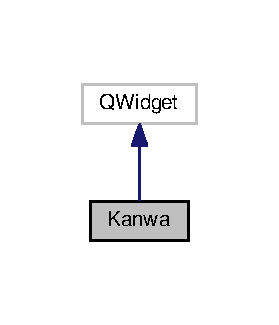
\includegraphics[width=134pt]{class_kanwa__inherit__graph}
\end{center}
\end{figure}


Diagram współpracy dla Kanwa\-:
\nopagebreak
\begin{figure}[H]
\begin{center}
\leavevmode
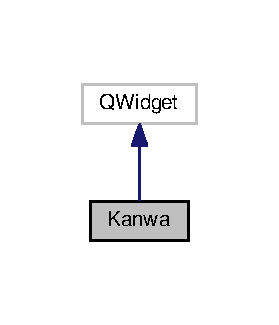
\includegraphics[width=134pt]{class_kanwa__coll__graph}
\end{center}
\end{figure}
\subsection*{Metody publiczne}
\begin{DoxyCompactItemize}
\item 
\hyperlink{class_kanwa_a6a634418b76abed84199abe8d2680c91}{Kanwa} (Q\-Widget $\ast$w\-Rodzic=0\-L)
\begin{DoxyCompactList}\small\item\em Konstruktor. \end{DoxyCompactList}\end{DoxyCompactItemize}


\subsection{Opis szczegółowy}


Definicja w linii 22 pliku ciecz.\-hh.



\subsection{Dokumentacja konstruktora i destruktora}
\hypertarget{class_kanwa_a6a634418b76abed84199abe8d2680c91}{\index{Kanwa@{Kanwa}!Kanwa@{Kanwa}}
\index{Kanwa@{Kanwa}!Kanwa@{Kanwa}}
\subsubsection[{Kanwa}]{\setlength{\rightskip}{0pt plus 5cm}Kanwa\-::\-Kanwa (
\begin{DoxyParamCaption}
\item[{Q\-Widget $\ast$}]{w\-Rodzic = {\ttfamily 0L}}
\end{DoxyParamCaption}
)}}\label{class_kanwa_a6a634418b76abed84199abe8d2680c91}

\begin{DoxyParams}[1]{Parametry}
\mbox{\tt in,out}  & {\em w\-Rodzic} & -\/ wskaznik na rodzica \\
\hline
\end{DoxyParams}


Definicja w linii 68 pliku ciecz.\-cpp.



Dokumentacja dla tej klasy została wygenerowana z plików\-:\begin{DoxyCompactItemize}
\item 
\hyperlink{ciecz_8hh}{ciecz.\-hh}\item 
\hyperlink{ciecz_8cpp}{ciecz.\-cpp}\end{DoxyCompactItemize}

\hypertarget{class_okno_glowne}{\section{Dokumentacja klasy Okno\-Glowne}
\label{class_okno_glowne}\index{Okno\-Glowne@{Okno\-Glowne}}
}


Klasa modelujaca głowne okno aplikacji.  




{\ttfamily \#include $<$okno\-\_\-glowne.\-hh$>$}



Diagram dziedziczenia dla Okno\-Glowne\nopagebreak
\begin{figure}[H]
\begin{center}
\leavevmode
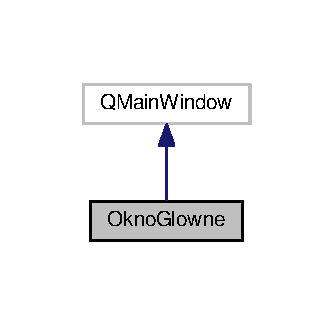
\includegraphics[width=160pt]{class_okno_glowne__inherit__graph}
\end{center}
\end{figure}


Diagram współpracy dla Okno\-Glowne\-:\nopagebreak
\begin{figure}[H]
\begin{center}
\leavevmode
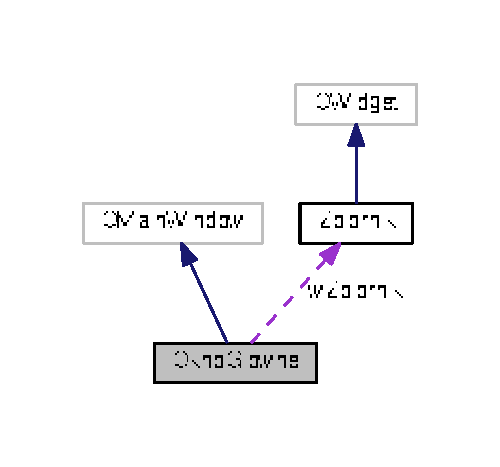
\includegraphics[width=293pt]{class_okno_glowne__coll__graph}
\end{center}
\end{figure}
\subsection*{Sloty publiczne}
\begin{DoxyCompactItemize}
\item 
void \hyperlink{class_okno_glowne_a2a49d3696ef8a42325313842768f2c92}{Gdy\-Odpowiedni\-Czas} ()
\begin{DoxyCompactList}\small\item\em Slot odpowiadajacy za aktualizacje danych. . \end{DoxyCompactList}\item 
void \hyperlink{class_okno_glowne_a2a59f13292adfead4ac821780220044a}{Gdy\-Napis} (const Q\-String \&)
\begin{DoxyCompactList}\small\item\em Slot odpowiadajacy za wyswietlenie napisu po otrzymaniu sygnalu. \end{DoxyCompactList}\item 
void \hyperlink{class_okno_glowne_ac837b1f8c8b0288d07987e059966431b}{on\-\_\-play\-Button\-\_\-clicked} ()
\begin{DoxyCompactList}\small\item\em Slot odpowiadajacy za obsluge stanu play. \end{DoxyCompactList}\item 
void \hyperlink{class_okno_glowne_ae8bd560de9aa835ba8b194b8f7da094c}{on\-\_\-pause\-Button\-\_\-clicked} ()
\begin{DoxyCompactList}\small\item\em Slot odpowiadajacy za obsluge stanu pauza. \end{DoxyCompactList}\item 
void \hyperlink{class_okno_glowne_a63255adc6263a1ee6f67c96b91446b73}{on\-\_\-stop\-Button\-\_\-clicked} ()
\begin{DoxyCompactList}\small\item\em Slot odpowiadajacy za obsluge stanu stop. \end{DoxyCompactList}\item 
void \hyperlink{class_okno_glowne_aba5accbf5e231ba194ee0e966b8d7b15}{on\-\_\-load\-Button\-\_\-clicked} ()
\begin{DoxyCompactList}\small\item\em Slot odpowiadajacy za wczytanie danych z pliku. \end{DoxyCompactList}\item 
void \hyperlink{class_okno_glowne_a0c744f19fcf0e4bcd04a49502864e020}{on\-\_\-line\-Edit\-\_\-return\-Pressed} ()
\begin{DoxyCompactList}\small\item\em Slot odpowiadajacy za wczytanie danych z pliku. \end{DoxyCompactList}\item 
void \hyperlink{class_okno_glowne_a726ce3fbe89c3fb7364c39e99c0ad658}{on\-\_\-slider\-Szybkosc\-Sym\-\_\-value\-Changed} (int a)
\begin{DoxyCompactList}\small\item\em Slot odpowiadajacy za zmiane wartosci slidera. \end{DoxyCompactList}\item 
void \hyperlink{class_okno_glowne_a8ed8fc49c9c3d3e187639880ce286c88}{on\-\_\-action\-\_\-\-Save\-\_\-triggered} ()
\begin{DoxyCompactList}\small\item\em Slot odpowiadajacy za przycisniecie przycisku Save. \end{DoxyCompactList}\end{DoxyCompactItemize}
\subsection*{Sygnały}
\begin{DoxyCompactItemize}
\item 
void \hyperlink{class_okno_glowne_aa602a0c5a940f0af4ab7390bfc1a4b9d}{Zglos\-Napis} (const Q\-String \&)
\begin{DoxyCompactList}\small\item\em Sygnal zglaszajacy napis. \end{DoxyCompactList}\end{DoxyCompactItemize}
\subsection*{Metody publiczne}
\begin{DoxyCompactItemize}
\item 
\hyperlink{class_okno_glowne_a8dcfe4e0f18dfaf0c535c4549991b550}{Okno\-Glowne} (Q\-Widget $\ast$w\-Rodzic=N\-U\-L\-L)
\begin{DoxyCompactList}\small\item\em Konstruktor. \end{DoxyCompactList}\item 
virtual void \hyperlink{class_okno_glowne_a570c795e3829c3bd7896551c0624abe2}{paint\-Event} (Q\-Paint\-Event $\ast$event)
\begin{DoxyCompactList}\small\item\em Wirtualna metoda paint\-Event wyrysowujaca obiekty na ekranie. \end{DoxyCompactList}\item 
void \hyperlink{class_okno_glowne_a6062f76fdf15ad8bc0543cfd2a2fe150}{Zapisz\-Symulacje\-Do\-Pliku} ()
\begin{DoxyCompactList}\small\item\em Metoda zapisujaca aktualny stan symulacji do pliku. \end{DoxyCompactList}\item 
void \hyperlink{class_okno_glowne_a1b8098c27e9656235bb056aeb79a8ece}{Wczytaj\-Symulacje\-Z\-Pliku} (const std\-::string nazwa\-\_\-pliku)
\begin{DoxyCompactList}\small\item\em Metoda wczytujaca z pliku stan symulacji. \end{DoxyCompactList}\end{DoxyCompactItemize}
\subsection*{Atrybuty publiczne}
\begin{DoxyCompactItemize}
\item 
Q\-Timer \hyperlink{class_okno_glowne_a5d047f90666212f58e69d11af3285d9b}{\-\_\-\-Stoper}
\begin{DoxyCompactList}\small\item\em Miernik czasu. \end{DoxyCompactList}\end{DoxyCompactItemize}
\subsection*{Atrybuty prywatne}
\begin{DoxyCompactItemize}
\item 
\hyperlink{class_zbiornik}{Zbiornik} $\ast$ \hyperlink{class_okno_glowne_af2d1275209898ebdd5ab9de8ef78dffd}{w\-Zbiornik}
\begin{DoxyCompactList}\small\item\em Wskaznik na zbiornik. \end{DoxyCompactList}\item 
Q\-Menu\-Bar $\ast$ \hyperlink{class_okno_glowne_a5a87098d9d4bd868670f5a5e72023a0a}{menu\-Bar}
\begin{DoxyCompactList}\small\item\em Wskaznik na pasek menu. \end{DoxyCompactList}\item 
Q\-Action $\ast$ \hyperlink{class_okno_glowne_a2c2d825b6e5e0faa5eb368be4fc73b78}{action\-\_\-\-Save}
\begin{DoxyCompactList}\small\item\em Wskaznik na akcje przycisku menu Save. \end{DoxyCompactList}\item 
Q\-Action $\ast$ \hyperlink{class_okno_glowne_a579ef9901f57057368cb522ea5a9a5c3}{action\-\_\-\-Exit}
\begin{DoxyCompactList}\small\item\em Wskaznik na akcje przycisku menu Exit. \end{DoxyCompactList}\item 
Q\-Menu $\ast$ \hyperlink{class_okno_glowne_a1ba162db2d0b06b0f8963e61b3806875}{menu\-\_\-\-File}
\begin{DoxyCompactList}\small\item\em Wskaznik na akcje przycisku menu File. \end{DoxyCompactList}\item 
Q\-Menu $\ast$ \hyperlink{class_okno_glowne_a93afadd0ec22ce6a7e29acc5dd2423a2}{menu\-\_\-\-Edit}
\begin{DoxyCompactList}\small\item\em Wskaznik na akcje przycisku menu Edit. \end{DoxyCompactList}\item 
Q\-Menu $\ast$ \hyperlink{class_okno_glowne_ab17be6714913af0cdf4e7de7cb6210d1}{menu\-\_\-\-Help}
\begin{DoxyCompactList}\small\item\em Wskaznik na akcje przycisku menu Help. \end{DoxyCompactList}\item 
Q\-Status\-Bar $\ast$ \hyperlink{class_okno_glowne_a40a10989bc6b318ac24e2457d7adb53b}{status\-Bar}
\begin{DoxyCompactList}\small\item\em Wskaznik na pasek statusowy. \end{DoxyCompactList}\item 
Q\-Tool\-Bar $\ast$ \hyperlink{class_okno_glowne_a6a37dd1f32605092fff7feac712bf429}{tool\-Bar}
\begin{DoxyCompactList}\small\item\em Wskaznik na pasek narzedziowy. \end{DoxyCompactList}\item 
Q\-H\-Box\-Layout $\ast$ \hyperlink{class_okno_glowne_aacb5ddb6d0eb560a47917cc1b457239a}{horizontal\-Layout}
\begin{DoxyCompactList}\small\item\em Wskaznik na obszar do horyzontalnego rozmieszczenia przyciskow. \end{DoxyCompactList}\item 
Q\-Widget $\ast$ \hyperlink{class_okno_glowne_a12ac2d00b9ca186176ccc710a928a723}{horizontal\-Layout\-Widget}
\begin{DoxyCompactList}\small\item\em Wskaznik na widget odpowiedzialny za horyzontalne wyswietlenie przyciskow. \end{DoxyCompactList}\item 
Q\-Push\-Button $\ast$ \hyperlink{class_okno_glowne_a50f936486c1bc3b3278823a8eb90841e}{play\-Button}
\begin{DoxyCompactList}\small\item\em Wskaznik na przycisk play. \end{DoxyCompactList}\item 
Q\-Push\-Button $\ast$ \hyperlink{class_okno_glowne_a0dde8df8a49b8f47f17f8e748fd15967}{pause\-Button}
\begin{DoxyCompactList}\small\item\em Wskaznik na przycisk pause. \end{DoxyCompactList}\item 
Q\-Push\-Button $\ast$ \hyperlink{class_okno_glowne_a3051d73dc0e0a27dc30ada43cc6b63c4}{stop\-Button}
\begin{DoxyCompactList}\small\item\em Wskaznik na przycisk stop. \end{DoxyCompactList}\item 
Q\-Push\-Button $\ast$ \hyperlink{class_okno_glowne_accbadc3bc4d418cfe1bce2be61881917}{load\-Button}
\begin{DoxyCompactList}\small\item\em Wskaznik na przycisk Wczytaj. \end{DoxyCompactList}\item 
Q\-Slider $\ast$ \hyperlink{class_okno_glowne_a85328893065393400d5a0344004ca78b}{slider\-Szybkosc\-Sym}
\begin{DoxyCompactList}\small\item\em Wskaznik na slider. \end{DoxyCompactList}\item 
Q\-L\-C\-D\-Number $\ast$ \hyperlink{class_okno_glowne_ab100c00d4ba33d896fd0985ac366296a}{lcd\-Szybkosc\-Sym}
\begin{DoxyCompactList}\small\item\em Wskaznik na L\-C\-D z szybkoscia symulacji. \end{DoxyCompactList}\item 
Q\-Label $\ast$ \hyperlink{class_okno_glowne_ad7b0708ffdf61f3bef1349cc353a6c4e}{label\-Szybkosc\-Sym}
\begin{DoxyCompactList}\small\item\em Wskaznik na etykiete z szybkoscia symulacji. \end{DoxyCompactList}\item 
Q\-Label $\ast$ \hyperlink{class_okno_glowne_aca07e1dc5cbe30d6952f9b952073bb79}{label\-Czas\-Sym}
\begin{DoxyCompactList}\small\item\em Wskaznik na etykiete z czasem symulacji. \end{DoxyCompactList}\item 
Q\-L\-C\-D\-Number $\ast$ \hyperlink{class_okno_glowne_ab34fefe738e38b1b0d4ce764481cc0c6}{lcd\-Czas\-Sym}
\begin{DoxyCompactList}\small\item\em Wskaznik na L\-C\-D z czasem trwania symulacji. \end{DoxyCompactList}\item 
Q\-Label $\ast$ \hyperlink{class_okno_glowne_ab01460f1222d0ec2892abf21efb23078}{label\-Liczba\-Czasteczek}
\begin{DoxyCompactList}\small\item\em Wskaznik na etykiete z liczbe czasteczek. \end{DoxyCompactList}\item 
Q\-L\-C\-D\-Number $\ast$ \hyperlink{class_okno_glowne_adbdd9fc009725804e015d267dc8375dc}{lcd\-Liczba\-Czasteczek}
\begin{DoxyCompactList}\small\item\em Wskaznik na L\-C\-D z liczbe czasteczek. \end{DoxyCompactList}\item 
Q\-Line\-Edit $\ast$ \hyperlink{class_okno_glowne_a0112b8be70a26552b03f38fab43a3301}{line\-Edit}
\begin{DoxyCompactList}\small\item\em Wskaznik na linijke do wpisywania tekstu. \end{DoxyCompactList}\item 
double \hyperlink{class_okno_glowne_a6a0922607c0970ecdfe8adec7a773c7f}{\-\_\-old\-\_\-width}
\begin{DoxyCompactList}\small\item\em Stara szerokosc okienka. \end{DoxyCompactList}\item 
double \hyperlink{class_okno_glowne_a7dae1b25dbade179eb6dfc30ffeab14b}{\-\_\-old\-\_\-height}
\begin{DoxyCompactList}\small\item\em Stara wysokosc okienka. \end{DoxyCompactList}\end{DoxyCompactItemize}
\subsection*{Statyczne atrybuty prywatne}
\begin{DoxyCompactItemize}
\item 
static int \hyperlink{class_okno_glowne_ae615cbd9c9f9ab06b365c4692ff68729}{licznik\-\_\-plikow}
\begin{DoxyCompactList}\small\item\em Sluzy do generowania unikatowych nazw plikow wyjsciowych. \end{DoxyCompactList}\end{DoxyCompactItemize}


\subsection{Opis szczegółowy}
Dzieki tej klasie wyswietlane jest okno glowne aplikacji. 

Definicja w linii 68 pliku okno\-\_\-glowne.\-hh.



\subsection{Dokumentacja konstruktora i destruktora}
\hypertarget{class_okno_glowne_a8dcfe4e0f18dfaf0c535c4549991b550}{\index{Okno\-Glowne@{Okno\-Glowne}!Okno\-Glowne@{Okno\-Glowne}}
\index{Okno\-Glowne@{Okno\-Glowne}!OknoGlowne@{Okno\-Glowne}}
\subsubsection[{Okno\-Glowne}]{\setlength{\rightskip}{0pt plus 5cm}Okno\-Glowne\-::\-Okno\-Glowne (
\begin{DoxyParamCaption}
\item[{Q\-Widget $\ast$}]{w\-Rodzic = {\ttfamily NULL}}
\end{DoxyParamCaption}
)}}\label{class_okno_glowne_a8dcfe4e0f18dfaf0c535c4549991b550}
Konstruktor parametryczny. 
\begin{DoxyParams}[1]{Parametry}
\mbox{\tt in,out}  & {\em w\-Rodzic} & -\/ wskaznik na rodzica \\
\hline
\end{DoxyParams}


Definicja w linii 16 pliku okno\-\_\-glowne.\-cpp.



Oto graf wywołań dla tej funkcji\-:\nopagebreak
\begin{figure}[H]
\begin{center}
\leavevmode
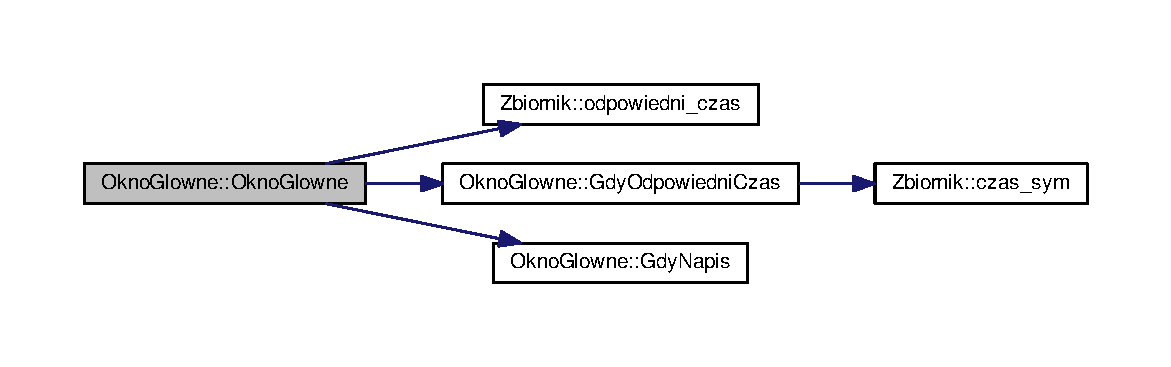
\includegraphics[width=350pt]{class_okno_glowne_a8dcfe4e0f18dfaf0c535c4549991b550_cgraph}
\end{center}
\end{figure}




\subsection{Dokumentacja funkcji składowych}
\hypertarget{class_okno_glowne_a2a59f13292adfead4ac821780220044a}{\index{Okno\-Glowne@{Okno\-Glowne}!Gdy\-Napis@{Gdy\-Napis}}
\index{Gdy\-Napis@{Gdy\-Napis}!OknoGlowne@{Okno\-Glowne}}
\subsubsection[{Gdy\-Napis}]{\setlength{\rightskip}{0pt plus 5cm}void Okno\-Glowne\-::\-Gdy\-Napis (
\begin{DoxyParamCaption}
\item[{const Q\-String \&}]{Napis}
\end{DoxyParamCaption}
)\hspace{0.3cm}{\ttfamily [slot]}}}\label{class_okno_glowne_a2a59f13292adfead4ac821780220044a}
Odpowiada za wyswietlenie napisu na belce statusowej. 
\begin{DoxyParams}[1]{Parametry}
\mbox{\tt in}  & {\em Napis} & -\/ napis do wyswietlenia \\
\hline
\end{DoxyParams}


Definicja w linii 223 pliku okno\-\_\-glowne.\-cpp.



Oto graf wywoływań tej funkcji\-:\nopagebreak
\begin{figure}[H]
\begin{center}
\leavevmode
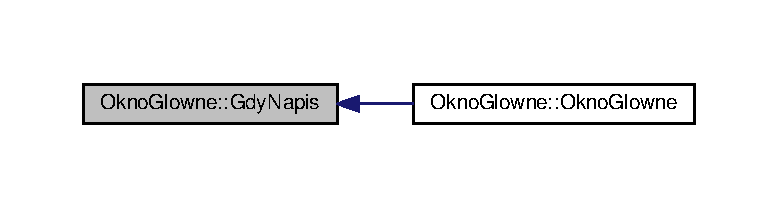
\includegraphics[width=350pt]{class_okno_glowne_a2a59f13292adfead4ac821780220044a_icgraph}
\end{center}
\end{figure}


\hypertarget{class_okno_glowne_a2a49d3696ef8a42325313842768f2c92}{\index{Okno\-Glowne@{Okno\-Glowne}!Gdy\-Odpowiedni\-Czas@{Gdy\-Odpowiedni\-Czas}}
\index{Gdy\-Odpowiedni\-Czas@{Gdy\-Odpowiedni\-Czas}!OknoGlowne@{Okno\-Glowne}}
\subsubsection[{Gdy\-Odpowiedni\-Czas}]{\setlength{\rightskip}{0pt plus 5cm}void Okno\-Glowne\-::\-Gdy\-Odpowiedni\-Czas (
\begin{DoxyParamCaption}
{}
\end{DoxyParamCaption}
)\hspace{0.3cm}{\ttfamily [slot]}}}\label{class_okno_glowne_a2a49d3696ef8a42325313842768f2c92}
Odpowiada za uaktualnienie okienka w odpowiednich momentach. 

Definicja w linii 215 pliku okno\-\_\-glowne.\-cpp.



Oto graf wywoływań tej funkcji\-:\nopagebreak
\begin{figure}[H]
\begin{center}
\leavevmode
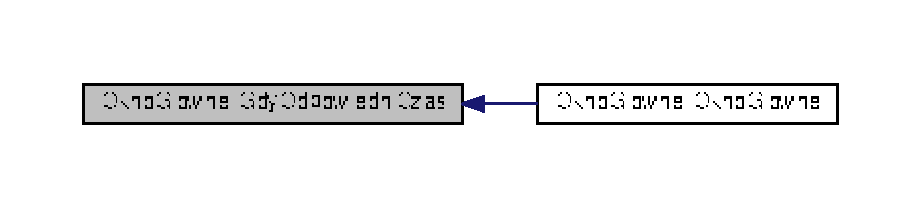
\includegraphics[width=350pt]{class_okno_glowne_a2a49d3696ef8a42325313842768f2c92_icgraph}
\end{center}
\end{figure}


\hypertarget{class_okno_glowne_a8ed8fc49c9c3d3e187639880ce286c88}{\index{Okno\-Glowne@{Okno\-Glowne}!on\-\_\-action\-\_\-\-Save\-\_\-triggered@{on\-\_\-action\-\_\-\-Save\-\_\-triggered}}
\index{on\-\_\-action\-\_\-\-Save\-\_\-triggered@{on\-\_\-action\-\_\-\-Save\-\_\-triggered}!OknoGlowne@{Okno\-Glowne}}
\subsubsection[{on\-\_\-action\-\_\-\-Save\-\_\-triggered}]{\setlength{\rightskip}{0pt plus 5cm}void Okno\-Glowne\-::on\-\_\-action\-\_\-\-Save\-\_\-triggered (
\begin{DoxyParamCaption}
{}
\end{DoxyParamCaption}
)\hspace{0.3cm}{\ttfamily [slot]}}}\label{class_okno_glowne_a8ed8fc49c9c3d3e187639880ce286c88}
Odpowiada za wykonanie odpowiednich czynnosci po przycisnieciu Save. 

Definicja w linii 204 pliku okno\-\_\-glowne.\-cpp.



Oto graf wywołań dla tej funkcji\-:\nopagebreak
\begin{figure}[H]
\begin{center}
\leavevmode
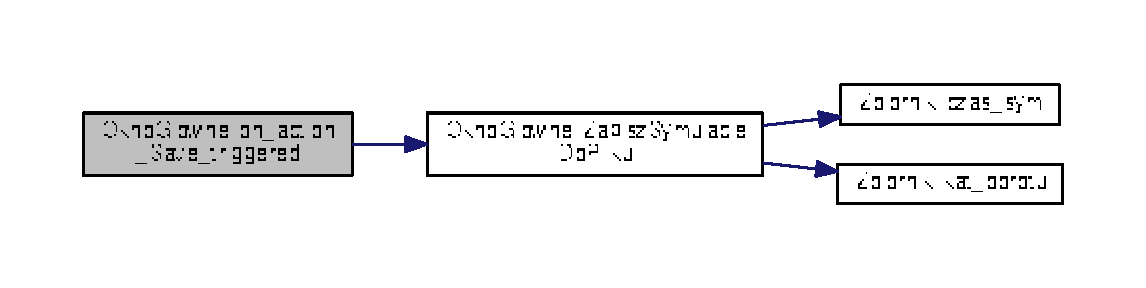
\includegraphics[width=350pt]{class_okno_glowne_a8ed8fc49c9c3d3e187639880ce286c88_cgraph}
\end{center}
\end{figure}


\hypertarget{class_okno_glowne_a0c744f19fcf0e4bcd04a49502864e020}{\index{Okno\-Glowne@{Okno\-Glowne}!on\-\_\-line\-Edit\-\_\-return\-Pressed@{on\-\_\-line\-Edit\-\_\-return\-Pressed}}
\index{on\-\_\-line\-Edit\-\_\-return\-Pressed@{on\-\_\-line\-Edit\-\_\-return\-Pressed}!OknoGlowne@{Okno\-Glowne}}
\subsubsection[{on\-\_\-line\-Edit\-\_\-return\-Pressed}]{\setlength{\rightskip}{0pt plus 5cm}void Okno\-Glowne\-::on\-\_\-line\-Edit\-\_\-return\-Pressed (
\begin{DoxyParamCaption}
{}
\end{DoxyParamCaption}
)\hspace{0.3cm}{\ttfamily [slot]}}}\label{class_okno_glowne_a0c744f19fcf0e4bcd04a49502864e020}
Odpowiada za wczytanie danych z pliku. 

Definicja w linii 191 pliku okno\-\_\-glowne.\-cpp.



Oto graf wywołań dla tej funkcji\-:
\nopagebreak
\begin{figure}[H]
\begin{center}
\leavevmode
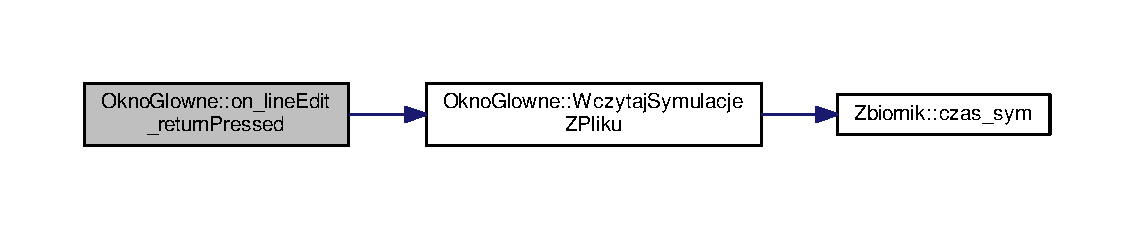
\includegraphics[width=350pt]{class_okno_glowne_a0c744f19fcf0e4bcd04a49502864e020_cgraph}
\end{center}
\end{figure}


\hypertarget{class_okno_glowne_aba5accbf5e231ba194ee0e966b8d7b15}{\index{Okno\-Glowne@{Okno\-Glowne}!on\-\_\-load\-Button\-\_\-clicked@{on\-\_\-load\-Button\-\_\-clicked}}
\index{on\-\_\-load\-Button\-\_\-clicked@{on\-\_\-load\-Button\-\_\-clicked}!OknoGlowne@{Okno\-Glowne}}
\subsubsection[{on\-\_\-load\-Button\-\_\-clicked}]{\setlength{\rightskip}{0pt plus 5cm}void Okno\-Glowne\-::on\-\_\-load\-Button\-\_\-clicked (
\begin{DoxyParamCaption}
{}
\end{DoxyParamCaption}
)\hspace{0.3cm}{\ttfamily [slot]}}}\label{class_okno_glowne_aba5accbf5e231ba194ee0e966b8d7b15}
Odpowiada za wczytanie danych z pliku. 

Definicja w linii 185 pliku okno\-\_\-glowne.\-cpp.



Oto graf wywołań dla tej funkcji\-:\nopagebreak
\begin{figure}[H]
\begin{center}
\leavevmode
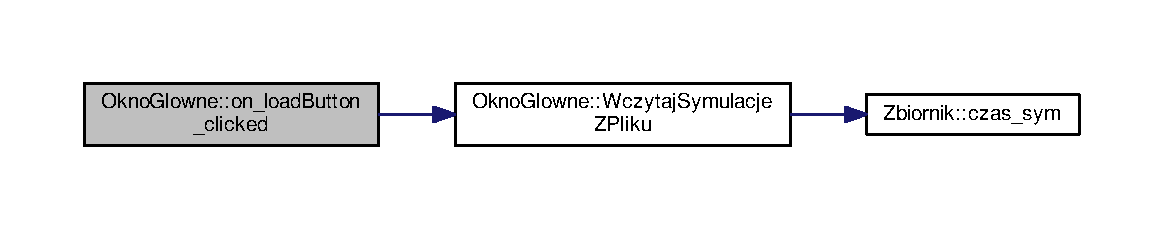
\includegraphics[width=350pt]{class_okno_glowne_aba5accbf5e231ba194ee0e966b8d7b15_cgraph}
\end{center}
\end{figure}


\hypertarget{class_okno_glowne_ae8bd560de9aa835ba8b194b8f7da094c}{\index{Okno\-Glowne@{Okno\-Glowne}!on\-\_\-pause\-Button\-\_\-clicked@{on\-\_\-pause\-Button\-\_\-clicked}}
\index{on\-\_\-pause\-Button\-\_\-clicked@{on\-\_\-pause\-Button\-\_\-clicked}!OknoGlowne@{Okno\-Glowne}}
\subsubsection[{on\-\_\-pause\-Button\-\_\-clicked}]{\setlength{\rightskip}{0pt plus 5cm}void Okno\-Glowne\-::on\-\_\-pause\-Button\-\_\-clicked (
\begin{DoxyParamCaption}
{}
\end{DoxyParamCaption}
)\hspace{0.3cm}{\ttfamily [slot]}}}\label{class_okno_glowne_ae8bd560de9aa835ba8b194b8f7da094c}
Odpowiada za wykonanie odpowiednich czynnosci w trakcie stanu pauza. 

Definicja w linii 177 pliku okno\-\_\-glowne.\-cpp.

\hypertarget{class_okno_glowne_ac837b1f8c8b0288d07987e059966431b}{\index{Okno\-Glowne@{Okno\-Glowne}!on\-\_\-play\-Button\-\_\-clicked@{on\-\_\-play\-Button\-\_\-clicked}}
\index{on\-\_\-play\-Button\-\_\-clicked@{on\-\_\-play\-Button\-\_\-clicked}!OknoGlowne@{Okno\-Glowne}}
\subsubsection[{on\-\_\-play\-Button\-\_\-clicked}]{\setlength{\rightskip}{0pt plus 5cm}void Okno\-Glowne\-::on\-\_\-play\-Button\-\_\-clicked (
\begin{DoxyParamCaption}
{}
\end{DoxyParamCaption}
)\hspace{0.3cm}{\ttfamily [slot]}}}\label{class_okno_glowne_ac837b1f8c8b0288d07987e059966431b}
Odpowiada za wykonanie odpowiednich czynnosci w trakcie stanu play. 

Definicja w linii 167 pliku okno\-\_\-glowne.\-cpp.



Oto graf wywołań dla tej funkcji\-:\nopagebreak
\begin{figure}[H]
\begin{center}
\leavevmode
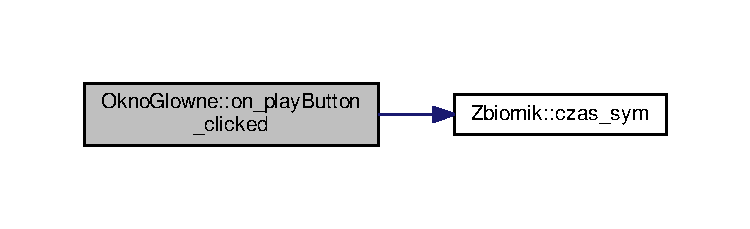
\includegraphics[width=350pt]{class_okno_glowne_ac837b1f8c8b0288d07987e059966431b_cgraph}
\end{center}
\end{figure}


\hypertarget{class_okno_glowne_a726ce3fbe89c3fb7364c39e99c0ad658}{\index{Okno\-Glowne@{Okno\-Glowne}!on\-\_\-slider\-Szybkosc\-Sym\-\_\-value\-Changed@{on\-\_\-slider\-Szybkosc\-Sym\-\_\-value\-Changed}}
\index{on\-\_\-slider\-Szybkosc\-Sym\-\_\-value\-Changed@{on\-\_\-slider\-Szybkosc\-Sym\-\_\-value\-Changed}!OknoGlowne@{Okno\-Glowne}}
\subsubsection[{on\-\_\-slider\-Szybkosc\-Sym\-\_\-value\-Changed}]{\setlength{\rightskip}{0pt plus 5cm}void Okno\-Glowne\-::on\-\_\-slider\-Szybkosc\-Sym\-\_\-value\-Changed (
\begin{DoxyParamCaption}
\item[{int}]{a}
\end{DoxyParamCaption}
)\hspace{0.3cm}{\ttfamily [slot]}}}\label{class_okno_glowne_a726ce3fbe89c3fb7364c39e99c0ad658}
Odpowiada za wykonanie odpowiednich czynnosci po zmianie wartosci slidera. 

Definicja w linii 197 pliku okno\-\_\-glowne.\-cpp.



Oto graf wywołań dla tej funkcji\-:\nopagebreak
\begin{figure}[H]
\begin{center}
\leavevmode
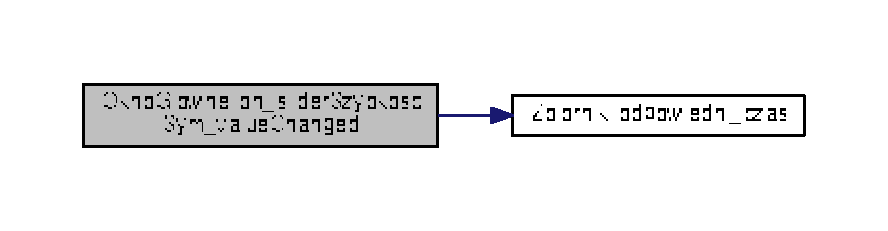
\includegraphics[width=350pt]{class_okno_glowne_a726ce3fbe89c3fb7364c39e99c0ad658_cgraph}
\end{center}
\end{figure}


\hypertarget{class_okno_glowne_a63255adc6263a1ee6f67c96b91446b73}{\index{Okno\-Glowne@{Okno\-Glowne}!on\-\_\-stop\-Button\-\_\-clicked@{on\-\_\-stop\-Button\-\_\-clicked}}
\index{on\-\_\-stop\-Button\-\_\-clicked@{on\-\_\-stop\-Button\-\_\-clicked}!OknoGlowne@{Okno\-Glowne}}
\subsubsection[{on\-\_\-stop\-Button\-\_\-clicked}]{\setlength{\rightskip}{0pt plus 5cm}void Okno\-Glowne\-::on\-\_\-stop\-Button\-\_\-clicked (
\begin{DoxyParamCaption}
{}
\end{DoxyParamCaption}
)\hspace{0.3cm}{\ttfamily [slot]}}}\label{class_okno_glowne_a63255adc6263a1ee6f67c96b91446b73}
Odpowiada za wykonanie odpowiednich czynnosci w trakcie stanu stop. 

Definicja w linii 181 pliku okno\-\_\-glowne.\-cpp.

\hypertarget{class_okno_glowne_a570c795e3829c3bd7896551c0624abe2}{\index{Okno\-Glowne@{Okno\-Glowne}!paint\-Event@{paint\-Event}}
\index{paint\-Event@{paint\-Event}!OknoGlowne@{Okno\-Glowne}}
\subsubsection[{paint\-Event}]{\setlength{\rightskip}{0pt plus 5cm}void Okno\-Glowne\-::paint\-Event (
\begin{DoxyParamCaption}
\item[{Q\-Paint\-Event $\ast$}]{event}
\end{DoxyParamCaption}
)\hspace{0.3cm}{\ttfamily [virtual]}}}\label{class_okno_glowne_a570c795e3829c3bd7896551c0624abe2}
Odziedziczona wirtualna metoda paint\-Event. Rysuje zbiornik i przyciski w nowym miejscu. 
\begin{DoxyParams}[1]{Parametry}
\mbox{\tt in,out}  & {\em event} & -\/ wskaznik obiekt klasy Q\-Paint\-Event \\
\hline
\end{DoxyParams}


Definicja w linii 227 pliku okno\-\_\-glowne.\-cpp.



Oto graf wywołań dla tej funkcji\-:\nopagebreak
\begin{figure}[H]
\begin{center}
\leavevmode
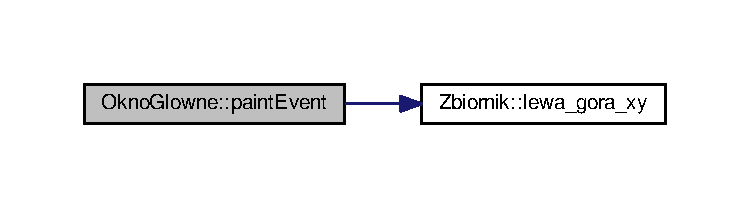
\includegraphics[width=350pt]{class_okno_glowne_a570c795e3829c3bd7896551c0624abe2_cgraph}
\end{center}
\end{figure}


\hypertarget{class_okno_glowne_a1b8098c27e9656235bb056aeb79a8ece}{\index{Okno\-Glowne@{Okno\-Glowne}!Wczytaj\-Symulacje\-Z\-Pliku@{Wczytaj\-Symulacje\-Z\-Pliku}}
\index{Wczytaj\-Symulacje\-Z\-Pliku@{Wczytaj\-Symulacje\-Z\-Pliku}!OknoGlowne@{Okno\-Glowne}}
\subsubsection[{Wczytaj\-Symulacje\-Z\-Pliku}]{\setlength{\rightskip}{0pt plus 5cm}void Okno\-Glowne\-::\-Wczytaj\-Symulacje\-Z\-Pliku (
\begin{DoxyParamCaption}
\item[{const std\-::string}]{nazwa\-\_\-pliku}
\end{DoxyParamCaption}
)}}\label{class_okno_glowne_a1b8098c27e9656235bb056aeb79a8ece}
Wczytuje stan symulacji (czas, liczba czasteczek, dane czasteczek). 

Definicja w linii 266 pliku okno\-\_\-glowne.\-cpp.



Oto graf wywołań dla tej funkcji\-:\nopagebreak
\begin{figure}[H]
\begin{center}
\leavevmode
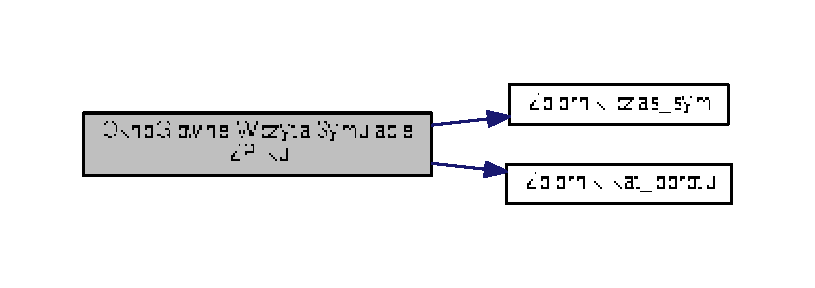
\includegraphics[width=350pt]{class_okno_glowne_a1b8098c27e9656235bb056aeb79a8ece_cgraph}
\end{center}
\end{figure}




Oto graf wywoływań tej funkcji\-:
\nopagebreak
\begin{figure}[H]
\begin{center}
\leavevmode
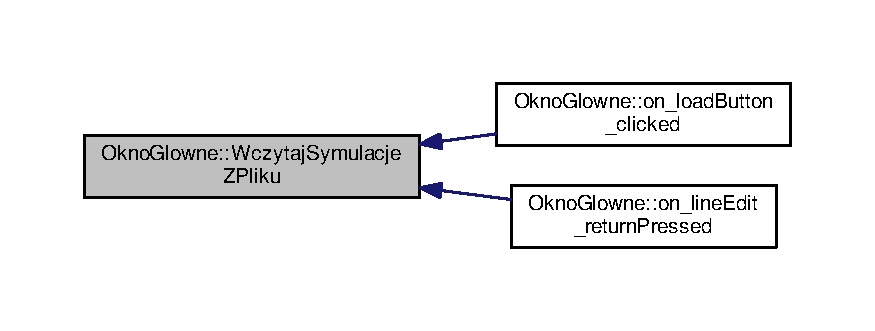
\includegraphics[width=350pt]{class_okno_glowne_a1b8098c27e9656235bb056aeb79a8ece_icgraph}
\end{center}
\end{figure}


\hypertarget{class_okno_glowne_a6062f76fdf15ad8bc0543cfd2a2fe150}{\index{Okno\-Glowne@{Okno\-Glowne}!Zapisz\-Symulacje\-Do\-Pliku@{Zapisz\-Symulacje\-Do\-Pliku}}
\index{Zapisz\-Symulacje\-Do\-Pliku@{Zapisz\-Symulacje\-Do\-Pliku}!OknoGlowne@{Okno\-Glowne}}
\subsubsection[{Zapisz\-Symulacje\-Do\-Pliku}]{\setlength{\rightskip}{0pt plus 5cm}void Okno\-Glowne\-::\-Zapisz\-Symulacje\-Do\-Pliku (
\begin{DoxyParamCaption}
{}
\end{DoxyParamCaption}
)}}\label{class_okno_glowne_a6062f76fdf15ad8bc0543cfd2a2fe150}
Zapisuje aktualny stan symulacji (czas, liczba czasteczek, dane czasteczek) do pliku. 

Definicja w linii 243 pliku okno\-\_\-glowne.\-cpp.



Oto graf wywołań dla tej funkcji\-:\nopagebreak
\begin{figure}[H]
\begin{center}
\leavevmode
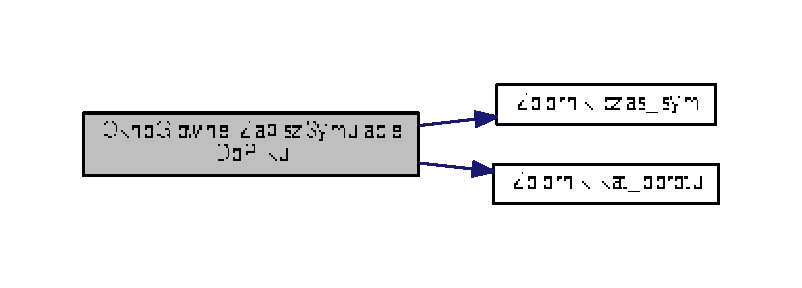
\includegraphics[width=350pt]{class_okno_glowne_a6062f76fdf15ad8bc0543cfd2a2fe150_cgraph}
\end{center}
\end{figure}




Oto graf wywoływań tej funkcji\-:\nopagebreak
\begin{figure}[H]
\begin{center}
\leavevmode
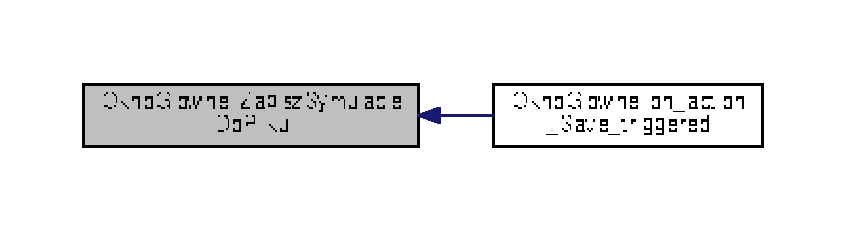
\includegraphics[width=350pt]{class_okno_glowne_a6062f76fdf15ad8bc0543cfd2a2fe150_icgraph}
\end{center}
\end{figure}


\hypertarget{class_okno_glowne_aa602a0c5a940f0af4ab7390bfc1a4b9d}{\index{Okno\-Glowne@{Okno\-Glowne}!Zglos\-Napis@{Zglos\-Napis}}
\index{Zglos\-Napis@{Zglos\-Napis}!OknoGlowne@{Okno\-Glowne}}
\subsubsection[{Zglos\-Napis}]{\setlength{\rightskip}{0pt plus 5cm}void Okno\-Glowne\-::\-Zglos\-Napis (
\begin{DoxyParamCaption}
\item[{const Q\-String \&}]{\-\_\-t1}
\end{DoxyParamCaption}
)\hspace{0.3cm}{\ttfamily [signal]}}}\label{class_okno_glowne_aa602a0c5a940f0af4ab7390bfc1a4b9d}
Sygnal zglaszajacy napis do odpowiedniego slotu. 
\begin{DoxyParams}[1]{Parametry}
\mbox{\tt in}  & {\em \-\_\-t1} & -\/ napis do zgloszenia \\
\hline
\end{DoxyParams}


Definicja w linii 121 pliku moc\-\_\-okno\-\_\-glowne.\-cpp.



Oto graf wywoływań tej funkcji\-:\nopagebreak
\begin{figure}[H]
\begin{center}
\leavevmode
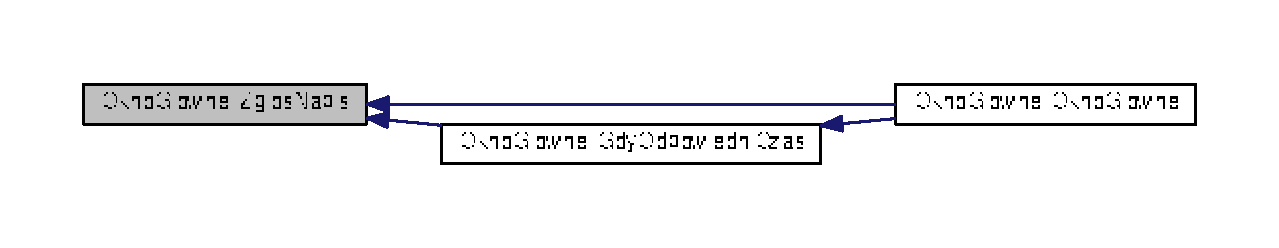
\includegraphics[width=350pt]{class_okno_glowne_aa602a0c5a940f0af4ab7390bfc1a4b9d_icgraph}
\end{center}
\end{figure}




\subsection{Dokumentacja atrybutów składowych}
\hypertarget{class_okno_glowne_a7dae1b25dbade179eb6dfc30ffeab14b}{\index{Okno\-Glowne@{Okno\-Glowne}!\-\_\-old\-\_\-height@{\-\_\-old\-\_\-height}}
\index{\-\_\-old\-\_\-height@{\-\_\-old\-\_\-height}!OknoGlowne@{Okno\-Glowne}}
\subsubsection[{\-\_\-old\-\_\-height}]{\setlength{\rightskip}{0pt plus 5cm}double Okno\-Glowne\-::\-\_\-old\-\_\-height\hspace{0.3cm}{\ttfamily [private]}}}\label{class_okno_glowne_a7dae1b25dbade179eb6dfc30ffeab14b}
Stara wysokosc okienka. 

Definicja w linii 367 pliku okno\-\_\-glowne.\-hh.

\hypertarget{class_okno_glowne_a6a0922607c0970ecdfe8adec7a773c7f}{\index{Okno\-Glowne@{Okno\-Glowne}!\-\_\-old\-\_\-width@{\-\_\-old\-\_\-width}}
\index{\-\_\-old\-\_\-width@{\-\_\-old\-\_\-width}!OknoGlowne@{Okno\-Glowne}}
\subsubsection[{\-\_\-old\-\_\-width}]{\setlength{\rightskip}{0pt plus 5cm}double Okno\-Glowne\-::\-\_\-old\-\_\-width\hspace{0.3cm}{\ttfamily [private]}}}\label{class_okno_glowne_a6a0922607c0970ecdfe8adec7a773c7f}
Stara szerokosc okienka. 

Definicja w linii 361 pliku okno\-\_\-glowne.\-hh.

\hypertarget{class_okno_glowne_a5d047f90666212f58e69d11af3285d9b}{\index{Okno\-Glowne@{Okno\-Glowne}!\-\_\-\-Stoper@{\-\_\-\-Stoper}}
\index{\-\_\-\-Stoper@{\-\_\-\-Stoper}!OknoGlowne@{Okno\-Glowne}}
\subsubsection[{\-\_\-\-Stoper}]{\setlength{\rightskip}{0pt plus 5cm}Q\-Timer Okno\-Glowne\-::\-\_\-\-Stoper}}\label{class_okno_glowne_a5d047f90666212f58e69d11af3285d9b}
Miernik czasu. 

Definicja w linii 353 pliku okno\-\_\-glowne.\-hh.

\hypertarget{class_okno_glowne_a579ef9901f57057368cb522ea5a9a5c3}{\index{Okno\-Glowne@{Okno\-Glowne}!action\-\_\-\-Exit@{action\-\_\-\-Exit}}
\index{action\-\_\-\-Exit@{action\-\_\-\-Exit}!OknoGlowne@{Okno\-Glowne}}
\subsubsection[{action\-\_\-\-Exit}]{\setlength{\rightskip}{0pt plus 5cm}Q\-Action$\ast$ Okno\-Glowne\-::action\-\_\-\-Exit\hspace{0.3cm}{\ttfamily [private]}}}\label{class_okno_glowne_a579ef9901f57057368cb522ea5a9a5c3}
Wskaznik na akcje przycisku menu Exit. 

Definicja w linii 212 pliku okno\-\_\-glowne.\-hh.

\hypertarget{class_okno_glowne_a2c2d825b6e5e0faa5eb368be4fc73b78}{\index{Okno\-Glowne@{Okno\-Glowne}!action\-\_\-\-Save@{action\-\_\-\-Save}}
\index{action\-\_\-\-Save@{action\-\_\-\-Save}!OknoGlowne@{Okno\-Glowne}}
\subsubsection[{action\-\_\-\-Save}]{\setlength{\rightskip}{0pt plus 5cm}Q\-Action$\ast$ Okno\-Glowne\-::action\-\_\-\-Save\hspace{0.3cm}{\ttfamily [private]}}}\label{class_okno_glowne_a2c2d825b6e5e0faa5eb368be4fc73b78}
Wskaznik na akcje przycisku menu Save. 

Definicja w linii 205 pliku okno\-\_\-glowne.\-hh.

\hypertarget{class_okno_glowne_aacb5ddb6d0eb560a47917cc1b457239a}{\index{Okno\-Glowne@{Okno\-Glowne}!horizontal\-Layout@{horizontal\-Layout}}
\index{horizontal\-Layout@{horizontal\-Layout}!OknoGlowne@{Okno\-Glowne}}
\subsubsection[{horizontal\-Layout}]{\setlength{\rightskip}{0pt plus 5cm}Q\-H\-Box\-Layout$\ast$ Okno\-Glowne\-::horizontal\-Layout\hspace{0.3cm}{\ttfamily [private]}}}\label{class_okno_glowne_aacb5ddb6d0eb560a47917cc1b457239a}
Wskaznik na obszar do horyzontalnego rozmieszczenia przyciskow. 

Definicja w linii 254 pliku okno\-\_\-glowne.\-hh.

\hypertarget{class_okno_glowne_a12ac2d00b9ca186176ccc710a928a723}{\index{Okno\-Glowne@{Okno\-Glowne}!horizontal\-Layout\-Widget@{horizontal\-Layout\-Widget}}
\index{horizontal\-Layout\-Widget@{horizontal\-Layout\-Widget}!OknoGlowne@{Okno\-Glowne}}
\subsubsection[{horizontal\-Layout\-Widget}]{\setlength{\rightskip}{0pt plus 5cm}Q\-Widget$\ast$ Okno\-Glowne\-::horizontal\-Layout\-Widget\hspace{0.3cm}{\ttfamily [private]}}}\label{class_okno_glowne_a12ac2d00b9ca186176ccc710a928a723}
Wskaznik na widget odpowiedzialny za horyzontalne wyswietlenie przyciskow. 

Definicja w linii 261 pliku okno\-\_\-glowne.\-hh.

\hypertarget{class_okno_glowne_aca07e1dc5cbe30d6952f9b952073bb79}{\index{Okno\-Glowne@{Okno\-Glowne}!label\-Czas\-Sym@{label\-Czas\-Sym}}
\index{label\-Czas\-Sym@{label\-Czas\-Sym}!OknoGlowne@{Okno\-Glowne}}
\subsubsection[{label\-Czas\-Sym}]{\setlength{\rightskip}{0pt plus 5cm}Q\-Label$\ast$ Okno\-Glowne\-::label\-Czas\-Sym\hspace{0.3cm}{\ttfamily [private]}}}\label{class_okno_glowne_aca07e1dc5cbe30d6952f9b952073bb79}
Etykieta dla czasu symulacji. 

Definicja w linii 317 pliku okno\-\_\-glowne.\-hh.

\hypertarget{class_okno_glowne_ab01460f1222d0ec2892abf21efb23078}{\index{Okno\-Glowne@{Okno\-Glowne}!label\-Liczba\-Czasteczek@{label\-Liczba\-Czasteczek}}
\index{label\-Liczba\-Czasteczek@{label\-Liczba\-Czasteczek}!OknoGlowne@{Okno\-Glowne}}
\subsubsection[{label\-Liczba\-Czasteczek}]{\setlength{\rightskip}{0pt plus 5cm}Q\-Label$\ast$ Okno\-Glowne\-::label\-Liczba\-Czasteczek\hspace{0.3cm}{\ttfamily [private]}}}\label{class_okno_glowne_ab01460f1222d0ec2892abf21efb23078}
Etykieta dla liczby symulowanych czasteczek. 

Definicja w linii 331 pliku okno\-\_\-glowne.\-hh.

\hypertarget{class_okno_glowne_ad7b0708ffdf61f3bef1349cc353a6c4e}{\index{Okno\-Glowne@{Okno\-Glowne}!label\-Szybkosc\-Sym@{label\-Szybkosc\-Sym}}
\index{label\-Szybkosc\-Sym@{label\-Szybkosc\-Sym}!OknoGlowne@{Okno\-Glowne}}
\subsubsection[{label\-Szybkosc\-Sym}]{\setlength{\rightskip}{0pt plus 5cm}Q\-Label$\ast$ Okno\-Glowne\-::label\-Szybkosc\-Sym\hspace{0.3cm}{\ttfamily [private]}}}\label{class_okno_glowne_ad7b0708ffdf61f3bef1349cc353a6c4e}
Etykieta dla szybkosci symulacji. 

Definicja w linii 310 pliku okno\-\_\-glowne.\-hh.

\hypertarget{class_okno_glowne_ab34fefe738e38b1b0d4ce764481cc0c6}{\index{Okno\-Glowne@{Okno\-Glowne}!lcd\-Czas\-Sym@{lcd\-Czas\-Sym}}
\index{lcd\-Czas\-Sym@{lcd\-Czas\-Sym}!OknoGlowne@{Okno\-Glowne}}
\subsubsection[{lcd\-Czas\-Sym}]{\setlength{\rightskip}{0pt plus 5cm}Q\-L\-C\-D\-Number$\ast$ Okno\-Glowne\-::lcd\-Czas\-Sym\hspace{0.3cm}{\ttfamily [private]}}}\label{class_okno_glowne_ab34fefe738e38b1b0d4ce764481cc0c6}
Wskaznik na L\-C\-D z szybkoscia symulacji. Wyswietla jej czas trwania. 

Definicja w linii 324 pliku okno\-\_\-glowne.\-hh.

\hypertarget{class_okno_glowne_adbdd9fc009725804e015d267dc8375dc}{\index{Okno\-Glowne@{Okno\-Glowne}!lcd\-Liczba\-Czasteczek@{lcd\-Liczba\-Czasteczek}}
\index{lcd\-Liczba\-Czasteczek@{lcd\-Liczba\-Czasteczek}!OknoGlowne@{Okno\-Glowne}}
\subsubsection[{lcd\-Liczba\-Czasteczek}]{\setlength{\rightskip}{0pt plus 5cm}Q\-L\-C\-D\-Number$\ast$ Okno\-Glowne\-::lcd\-Liczba\-Czasteczek\hspace{0.3cm}{\ttfamily [private]}}}\label{class_okno_glowne_adbdd9fc009725804e015d267dc8375dc}
Wyswietla liczbe symulowanych czasteczek. 

Definicja w linii 338 pliku okno\-\_\-glowne.\-hh.

\hypertarget{class_okno_glowne_ab100c00d4ba33d896fd0985ac366296a}{\index{Okno\-Glowne@{Okno\-Glowne}!lcd\-Szybkosc\-Sym@{lcd\-Szybkosc\-Sym}}
\index{lcd\-Szybkosc\-Sym@{lcd\-Szybkosc\-Sym}!OknoGlowne@{Okno\-Glowne}}
\subsubsection[{lcd\-Szybkosc\-Sym}]{\setlength{\rightskip}{0pt plus 5cm}Q\-L\-C\-D\-Number$\ast$ Okno\-Glowne\-::lcd\-Szybkosc\-Sym\hspace{0.3cm}{\ttfamily [private]}}}\label{class_okno_glowne_ab100c00d4ba33d896fd0985ac366296a}
Wskaznik na L\-C\-D z szybkoscia symulacji. Wyswietla jej szybkosc. 

Definicja w linii 303 pliku okno\-\_\-glowne.\-hh.

\hypertarget{class_okno_glowne_ae615cbd9c9f9ab06b365c4692ff68729}{\index{Okno\-Glowne@{Okno\-Glowne}!licznik\-\_\-plikow@{licznik\-\_\-plikow}}
\index{licznik\-\_\-plikow@{licznik\-\_\-plikow}!OknoGlowne@{Okno\-Glowne}}
\subsubsection[{licznik\-\_\-plikow}]{\setlength{\rightskip}{0pt plus 5cm}int Okno\-Glowne\-::licznik\-\_\-plikow\hspace{0.3cm}{\ttfamily [static]}, {\ttfamily [private]}}}\label{class_okno_glowne_ae615cbd9c9f9ab06b365c4692ff68729}
Sluzy do generowania unikatowych nazw plikow wyjsciowych. 

Definicja w linii 184 pliku okno\-\_\-glowne.\-hh.

\hypertarget{class_okno_glowne_a0112b8be70a26552b03f38fab43a3301}{\index{Okno\-Glowne@{Okno\-Glowne}!line\-Edit@{line\-Edit}}
\index{line\-Edit@{line\-Edit}!OknoGlowne@{Okno\-Glowne}}
\subsubsection[{line\-Edit}]{\setlength{\rightskip}{0pt plus 5cm}Q\-Line\-Edit$\ast$ Okno\-Glowne\-::line\-Edit\hspace{0.3cm}{\ttfamily [private]}}}\label{class_okno_glowne_a0112b8be70a26552b03f38fab43a3301}
Wskazuje linijke do wpisywania tekstu. 

Definicja w linii 345 pliku okno\-\_\-glowne.\-hh.

\hypertarget{class_okno_glowne_accbadc3bc4d418cfe1bce2be61881917}{\index{Okno\-Glowne@{Okno\-Glowne}!load\-Button@{load\-Button}}
\index{load\-Button@{load\-Button}!OknoGlowne@{Okno\-Glowne}}
\subsubsection[{load\-Button}]{\setlength{\rightskip}{0pt plus 5cm}Q\-Push\-Button$\ast$ Okno\-Glowne\-::load\-Button\hspace{0.3cm}{\ttfamily [private]}}}\label{class_okno_glowne_accbadc3bc4d418cfe1bce2be61881917}
Wskaznik na przycisk Wczytaj. Wczytuje symulacje. 

Definicja w linii 289 pliku okno\-\_\-glowne.\-hh.

\hypertarget{class_okno_glowne_a93afadd0ec22ce6a7e29acc5dd2423a2}{\index{Okno\-Glowne@{Okno\-Glowne}!menu\-\_\-\-Edit@{menu\-\_\-\-Edit}}
\index{menu\-\_\-\-Edit@{menu\-\_\-\-Edit}!OknoGlowne@{Okno\-Glowne}}
\subsubsection[{menu\-\_\-\-Edit}]{\setlength{\rightskip}{0pt plus 5cm}Q\-Menu$\ast$ Okno\-Glowne\-::menu\-\_\-\-Edit\hspace{0.3cm}{\ttfamily [private]}}}\label{class_okno_glowne_a93afadd0ec22ce6a7e29acc5dd2423a2}
Wskaznik na akcje przycisku menu Edit. 

Definicja w linii 226 pliku okno\-\_\-glowne.\-hh.

\hypertarget{class_okno_glowne_a1ba162db2d0b06b0f8963e61b3806875}{\index{Okno\-Glowne@{Okno\-Glowne}!menu\-\_\-\-File@{menu\-\_\-\-File}}
\index{menu\-\_\-\-File@{menu\-\_\-\-File}!OknoGlowne@{Okno\-Glowne}}
\subsubsection[{menu\-\_\-\-File}]{\setlength{\rightskip}{0pt plus 5cm}Q\-Menu$\ast$ Okno\-Glowne\-::menu\-\_\-\-File\hspace{0.3cm}{\ttfamily [private]}}}\label{class_okno_glowne_a1ba162db2d0b06b0f8963e61b3806875}
Wskaznik na akcje przycisku menu File. 

Definicja w linii 219 pliku okno\-\_\-glowne.\-hh.

\hypertarget{class_okno_glowne_ab17be6714913af0cdf4e7de7cb6210d1}{\index{Okno\-Glowne@{Okno\-Glowne}!menu\-\_\-\-Help@{menu\-\_\-\-Help}}
\index{menu\-\_\-\-Help@{menu\-\_\-\-Help}!OknoGlowne@{Okno\-Glowne}}
\subsubsection[{menu\-\_\-\-Help}]{\setlength{\rightskip}{0pt plus 5cm}Q\-Menu$\ast$ Okno\-Glowne\-::menu\-\_\-\-Help\hspace{0.3cm}{\ttfamily [private]}}}\label{class_okno_glowne_ab17be6714913af0cdf4e7de7cb6210d1}
Wskaznik na akcje przycisku menu Help. 

Definicja w linii 233 pliku okno\-\_\-glowne.\-hh.

\hypertarget{class_okno_glowne_a5a87098d9d4bd868670f5a5e72023a0a}{\index{Okno\-Glowne@{Okno\-Glowne}!menu\-Bar@{menu\-Bar}}
\index{menu\-Bar@{menu\-Bar}!OknoGlowne@{Okno\-Glowne}}
\subsubsection[{menu\-Bar}]{\setlength{\rightskip}{0pt plus 5cm}Q\-Menu\-Bar$\ast$ Okno\-Glowne\-::menu\-Bar\hspace{0.3cm}{\ttfamily [private]}}}\label{class_okno_glowne_a5a87098d9d4bd868670f5a5e72023a0a}
Wskaznik na pasek menu. 

Definicja w linii 198 pliku okno\-\_\-glowne.\-hh.

\hypertarget{class_okno_glowne_a0dde8df8a49b8f47f17f8e748fd15967}{\index{Okno\-Glowne@{Okno\-Glowne}!pause\-Button@{pause\-Button}}
\index{pause\-Button@{pause\-Button}!OknoGlowne@{Okno\-Glowne}}
\subsubsection[{pause\-Button}]{\setlength{\rightskip}{0pt plus 5cm}Q\-Push\-Button$\ast$ Okno\-Glowne\-::pause\-Button\hspace{0.3cm}{\ttfamily [private]}}}\label{class_okno_glowne_a0dde8df8a49b8f47f17f8e748fd15967}
Wskaznik na przycisk pause. Wstrzymuje symulacje. 

Definicja w linii 275 pliku okno\-\_\-glowne.\-hh.

\hypertarget{class_okno_glowne_a50f936486c1bc3b3278823a8eb90841e}{\index{Okno\-Glowne@{Okno\-Glowne}!play\-Button@{play\-Button}}
\index{play\-Button@{play\-Button}!OknoGlowne@{Okno\-Glowne}}
\subsubsection[{play\-Button}]{\setlength{\rightskip}{0pt plus 5cm}Q\-Push\-Button$\ast$ Okno\-Glowne\-::play\-Button\hspace{0.3cm}{\ttfamily [private]}}}\label{class_okno_glowne_a50f936486c1bc3b3278823a8eb90841e}
Wskaznik na przycisk play. Uruchamia symulacje. 

Definicja w linii 268 pliku okno\-\_\-glowne.\-hh.

\hypertarget{class_okno_glowne_a85328893065393400d5a0344004ca78b}{\index{Okno\-Glowne@{Okno\-Glowne}!slider\-Szybkosc\-Sym@{slider\-Szybkosc\-Sym}}
\index{slider\-Szybkosc\-Sym@{slider\-Szybkosc\-Sym}!OknoGlowne@{Okno\-Glowne}}
\subsubsection[{slider\-Szybkosc\-Sym}]{\setlength{\rightskip}{0pt plus 5cm}Q\-Slider$\ast$ Okno\-Glowne\-::slider\-Szybkosc\-Sym\hspace{0.3cm}{\ttfamily [private]}}}\label{class_okno_glowne_a85328893065393400d5a0344004ca78b}
Wskaznik na slider. Steruje szybkoscia symulacji. 

Definicja w linii 296 pliku okno\-\_\-glowne.\-hh.

\hypertarget{class_okno_glowne_a40a10989bc6b318ac24e2457d7adb53b}{\index{Okno\-Glowne@{Okno\-Glowne}!status\-Bar@{status\-Bar}}
\index{status\-Bar@{status\-Bar}!OknoGlowne@{Okno\-Glowne}}
\subsubsection[{status\-Bar}]{\setlength{\rightskip}{0pt plus 5cm}Q\-Status\-Bar$\ast$ Okno\-Glowne\-::status\-Bar\hspace{0.3cm}{\ttfamily [private]}}}\label{class_okno_glowne_a40a10989bc6b318ac24e2457d7adb53b}
Wskaznik na pasek statusowy. 

Definicja w linii 240 pliku okno\-\_\-glowne.\-hh.

\hypertarget{class_okno_glowne_a3051d73dc0e0a27dc30ada43cc6b63c4}{\index{Okno\-Glowne@{Okno\-Glowne}!stop\-Button@{stop\-Button}}
\index{stop\-Button@{stop\-Button}!OknoGlowne@{Okno\-Glowne}}
\subsubsection[{stop\-Button}]{\setlength{\rightskip}{0pt plus 5cm}Q\-Push\-Button$\ast$ Okno\-Glowne\-::stop\-Button\hspace{0.3cm}{\ttfamily [private]}}}\label{class_okno_glowne_a3051d73dc0e0a27dc30ada43cc6b63c4}
Wskaznik na przycisk stop. Zatrzymuje symulacje. 

Definicja w linii 282 pliku okno\-\_\-glowne.\-hh.

\hypertarget{class_okno_glowne_a6a37dd1f32605092fff7feac712bf429}{\index{Okno\-Glowne@{Okno\-Glowne}!tool\-Bar@{tool\-Bar}}
\index{tool\-Bar@{tool\-Bar}!OknoGlowne@{Okno\-Glowne}}
\subsubsection[{tool\-Bar}]{\setlength{\rightskip}{0pt plus 5cm}Q\-Tool\-Bar$\ast$ Okno\-Glowne\-::tool\-Bar\hspace{0.3cm}{\ttfamily [private]}}}\label{class_okno_glowne_a6a37dd1f32605092fff7feac712bf429}
Wskaznik na pasek narzedziowy. 

Definicja w linii 247 pliku okno\-\_\-glowne.\-hh.

\hypertarget{class_okno_glowne_af2d1275209898ebdd5ab9de8ef78dffd}{\index{Okno\-Glowne@{Okno\-Glowne}!w\-Zbiornik@{w\-Zbiornik}}
\index{w\-Zbiornik@{w\-Zbiornik}!OknoGlowne@{Okno\-Glowne}}
\subsubsection[{w\-Zbiornik}]{\setlength{\rightskip}{0pt plus 5cm}{\bf Zbiornik}$\ast$ Okno\-Glowne\-::w\-Zbiornik\hspace{0.3cm}{\ttfamily [private]}}}\label{class_okno_glowne_af2d1275209898ebdd5ab9de8ef78dffd}
Wskaznik na zbiornik. 

Definicja w linii 191 pliku okno\-\_\-glowne.\-hh.



Dokumentacja dla tej klasy została wygenerowana z plików\-:\begin{DoxyCompactItemize}
\item 
\hyperlink{okno__glowne_8hh}{okno\-\_\-glowne.\-hh}\item 
\hyperlink{moc__okno__glowne_8cpp}{moc\-\_\-okno\-\_\-glowne.\-cpp}\item 
\hyperlink{okno__glowne_8cpp}{okno\-\_\-glowne.\-cpp}\end{DoxyCompactItemize}

\hypertarget{class_vector}{}\section{Dokumentacja klasy Vector}
\label{class_vector}\index{Vector@{Vector}}


klasa \hyperlink{class_vector}{Vector}  




{\ttfamily \#include $<$vector.\+hh$>$}

\subsection*{Metody publiczne}
\begin{DoxyCompactItemize}
\item 
\hyperlink{class_vector_af3c1b04bfbb10e29433842202365a6c4}{Vector} (float \+\_\+x=0, float \+\_\+y=0)
\begin{DoxyCompactList}\small\item\em Współrzędne wektora. \end{DoxyCompactList}\item 
float \hyperlink{class_vector_ab2878a1bb81982dc83363646e25ce665}{get\+X} () const 
\begin{DoxyCompactList}\small\item\em zwraga pierwszą współrzędną wektora \end{DoxyCompactList}\item 
float \hyperlink{class_vector_a86293fe7a035979fd252be6071488b6a}{get\+Y} () const 
\begin{DoxyCompactList}\small\item\em pobiera drugą współrzędną wektora \end{DoxyCompactList}\item 
float \& \hyperlink{class_vector_aeca06c929d4ab3078a828723a88621e6}{get\+X} ()
\begin{DoxyCompactList}\small\item\em pobiera pierwszą współrzędną wektora \end{DoxyCompactList}\item 
float \& \hyperlink{class_vector_ab0cc77ce300a60de0ab734555886ad5d}{get\+Y} ()
\begin{DoxyCompactList}\small\item\em pobiera drugą współrzędną wektora \end{DoxyCompactList}\item 
\hyperlink{class_vector}{Vector} \& \hyperlink{class_vector_a4eeab5be24ee846de3012e67a4e34820}{operator+=} (const \hyperlink{class_vector}{Vector} \&\+\_\+v)
\begin{DoxyCompactList}\small\item\em operator dodawania \end{DoxyCompactList}\item 
\hyperlink{class_vector}{Vector} \& \hyperlink{class_vector_aaaf87dbf15cd9492aa0c11874ae5afef}{operator-\/=} (const \hyperlink{class_vector}{Vector} \&\+\_\+v)
\begin{DoxyCompactList}\small\item\em operator odejmowania \end{DoxyCompactList}\item 
\hyperlink{class_vector}{Vector} \& \hyperlink{class_vector_a91ebac6d502ca1d54645e7c711549867}{operator$\ast$=} (const float \&\+\_\+c)
\begin{DoxyCompactList}\small\item\em operator skalowania \end{DoxyCompactList}\item 
\hyperlink{class_vector}{Vector} \hyperlink{class_vector_aa78eb4c9e5ac236c89f0853eefa347ac}{operator+} (const \hyperlink{class_vector}{Vector} \&\+\_\+v) const 
\begin{DoxyCompactList}\small\item\em operator dodawania \end{DoxyCompactList}\item 
\hyperlink{class_vector}{Vector} \hyperlink{class_vector_a94b6fde82bef6532c00358a0af448fc1}{operator-\/} (const \hyperlink{class_vector}{Vector} \&\+\_\+v) const 
\begin{DoxyCompactList}\small\item\em operator odejmowania \end{DoxyCompactList}\item 
\hyperlink{class_vector}{Vector} \hyperlink{class_vector_a8f0e64ee9a688803b1efce30fb0b2869}{operator$\ast$} (const float \&\+\_\+c) const 
\begin{DoxyCompactList}\small\item\em operator skalowania \end{DoxyCompactList}\item 
\hyperlink{class_vector}{Vector} \& \hyperlink{class_vector_ad44f6d9721d9584e7f847e449df73e11}{operator=} (const \hyperlink{class_vector}{Vector} \&\+\_\+v)
\begin{DoxyCompactList}\small\item\em operator przypisania \end{DoxyCompactList}\item 
float \hyperlink{class_vector_a18d3f2110be751ac3a658016bd3dca69}{norm\+Squared} ()
\begin{DoxyCompactList}\small\item\em kwadrat normy \end{DoxyCompactList}\end{DoxyCompactItemize}
\subsection*{Atrybuty prywatne}
\begin{DoxyCompactItemize}
\item 
float \hyperlink{class_vector_aca49165049a1e21ae47afcfc078819ed}{x}
\item 
float \hyperlink{class_vector_a81be9102fca6d9beea3efef522c4c09d}{y}
\end{DoxyCompactItemize}
\subsection*{Przyjaciele}
\begin{DoxyCompactItemize}
\item 
std\+::ostream \& \hyperlink{class_vector_a7973d0032b0df4c3ab89e1da167b86a9}{operator$<$$<$} (std\+::ostream \&\+\_\+os, const \hyperlink{class_vector}{Vector} \&\+\_\+s)
\end{DoxyCompactItemize}


\subsection{Opis szczegółowy}
Posiada metody do obsługi dwuelementowych wektorów o współrzędnych typu float 

Definicja w linii 10 pliku vector.\+hh.



\subsection{Dokumentacja konstruktora i destruktora}
\hypertarget{class_vector_af3c1b04bfbb10e29433842202365a6c4}{}\index{Vector@{Vector}!Vector@{Vector}}
\index{Vector@{Vector}!Vector@{Vector}}
\subsubsection[{Vector}]{\setlength{\rightskip}{0pt plus 5cm}Vector\+::\+Vector (
\begin{DoxyParamCaption}
\item[{float}]{\+\_\+x = {\ttfamily 0}, }
\item[{float}]{\+\_\+y = {\ttfamily 0}}
\end{DoxyParamCaption}
)\hspace{0.3cm}{\ttfamily [inline]}}\label{class_vector_af3c1b04bfbb10e29433842202365a6c4}
konstruktor wektora

Ustawia współrzędne wektora 
\begin{DoxyParams}[1]{Parametry}
\mbox{\tt in}  & {\em \+\_\+x} & -\/ pierwsza współrzędna (domyślnie\+: 0) \\
\hline
\mbox{\tt in}  & {\em \+\_\+y} & -\/ druga współrzędna (domyślnie\+: 0) \\
\hline
\end{DoxyParams}


Definicja w linii 22 pliku vector.\+hh.



Oto graf wywoływań tej funkcji\+:\nopagebreak
\begin{figure}[H]
\begin{center}
\leavevmode
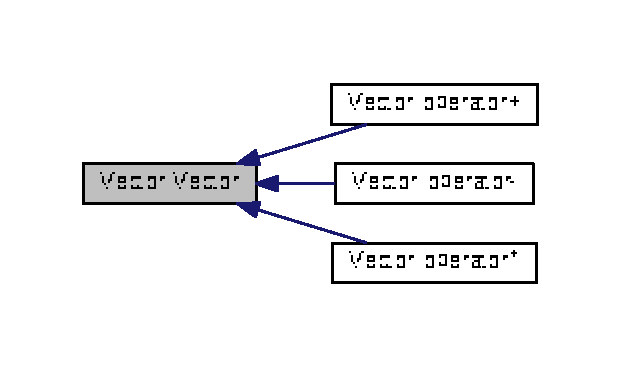
\includegraphics[width=298pt]{class_vector_af3c1b04bfbb10e29433842202365a6c4_icgraph}
\end{center}
\end{figure}




\subsection{Dokumentacja funkcji składowych}
\hypertarget{class_vector_ab2878a1bb81982dc83363646e25ce665}{}\index{Vector@{Vector}!get\+X@{get\+X}}
\index{get\+X@{get\+X}!Vector@{Vector}}
\subsubsection[{get\+X}]{\setlength{\rightskip}{0pt plus 5cm}float Vector\+::get\+X (
\begin{DoxyParamCaption}
{}
\end{DoxyParamCaption}
) const\hspace{0.3cm}{\ttfamily [inline]}}\label{class_vector_ab2878a1bb81982dc83363646e25ce665}
\begin{DoxyReturn}{Zwraca}
pierwsza współrzędna wektora jako stała 
\end{DoxyReturn}


Definicja w linii 27 pliku vector.\+hh.



Oto graf wywoływań tej funkcji\+:\nopagebreak
\begin{figure}[H]
\begin{center}
\leavevmode
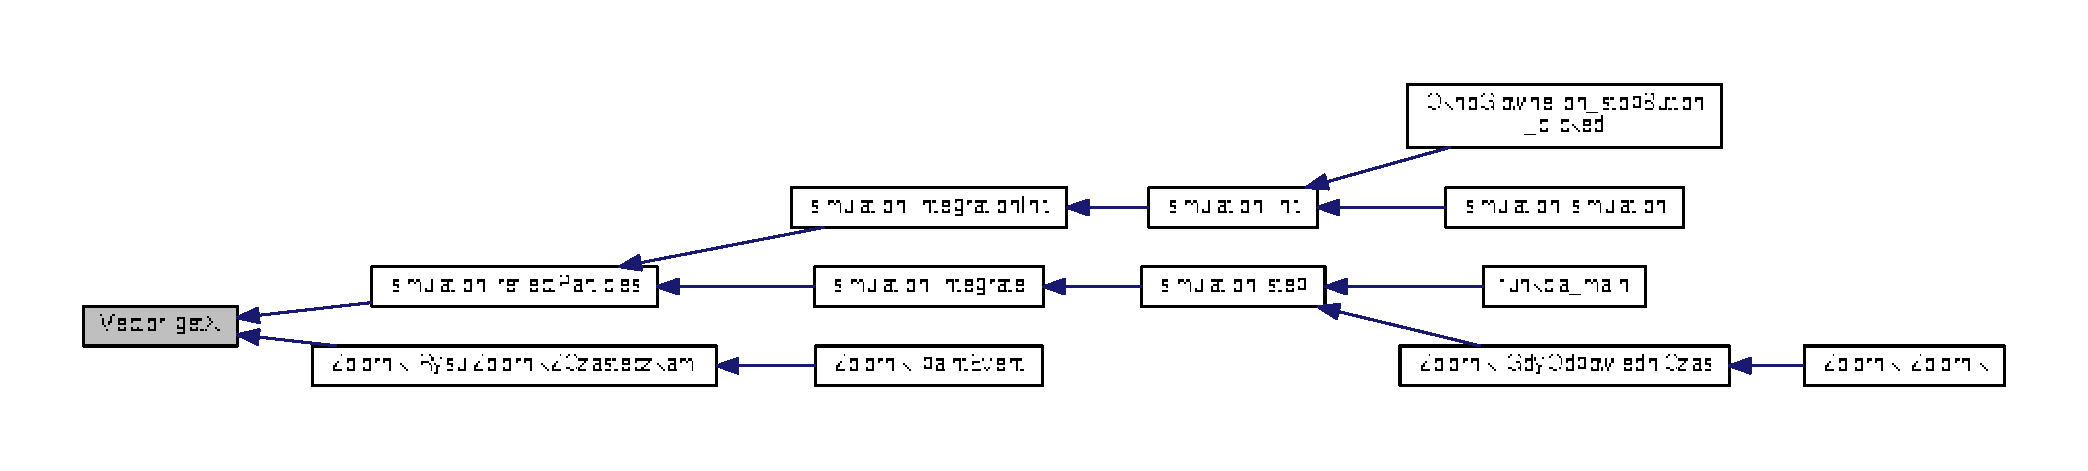
\includegraphics[width=350pt]{class_vector_ab2878a1bb81982dc83363646e25ce665_icgraph}
\end{center}
\end{figure}


\hypertarget{class_vector_aeca06c929d4ab3078a828723a88621e6}{}\index{Vector@{Vector}!get\+X@{get\+X}}
\index{get\+X@{get\+X}!Vector@{Vector}}
\subsubsection[{get\+X}]{\setlength{\rightskip}{0pt plus 5cm}float\& Vector\+::get\+X (
\begin{DoxyParamCaption}
{}
\end{DoxyParamCaption}
)\hspace{0.3cm}{\ttfamily [inline]}}\label{class_vector_aeca06c929d4ab3078a828723a88621e6}
\begin{DoxyReturn}{Zwraca}
pierwsza współrzędna wektora jako stała 
\end{DoxyReturn}


Definicja w linii 37 pliku vector.\+hh.

\hypertarget{class_vector_a86293fe7a035979fd252be6071488b6a}{}\index{Vector@{Vector}!get\+Y@{get\+Y}}
\index{get\+Y@{get\+Y}!Vector@{Vector}}
\subsubsection[{get\+Y}]{\setlength{\rightskip}{0pt plus 5cm}float Vector\+::get\+Y (
\begin{DoxyParamCaption}
{}
\end{DoxyParamCaption}
) const\hspace{0.3cm}{\ttfamily [inline]}}\label{class_vector_a86293fe7a035979fd252be6071488b6a}
\begin{DoxyReturn}{Zwraca}
druga współrzędna wektora jako stała 
\end{DoxyReturn}


Definicja w linii 32 pliku vector.\+hh.



Oto graf wywoływań tej funkcji\+:\nopagebreak
\begin{figure}[H]
\begin{center}
\leavevmode
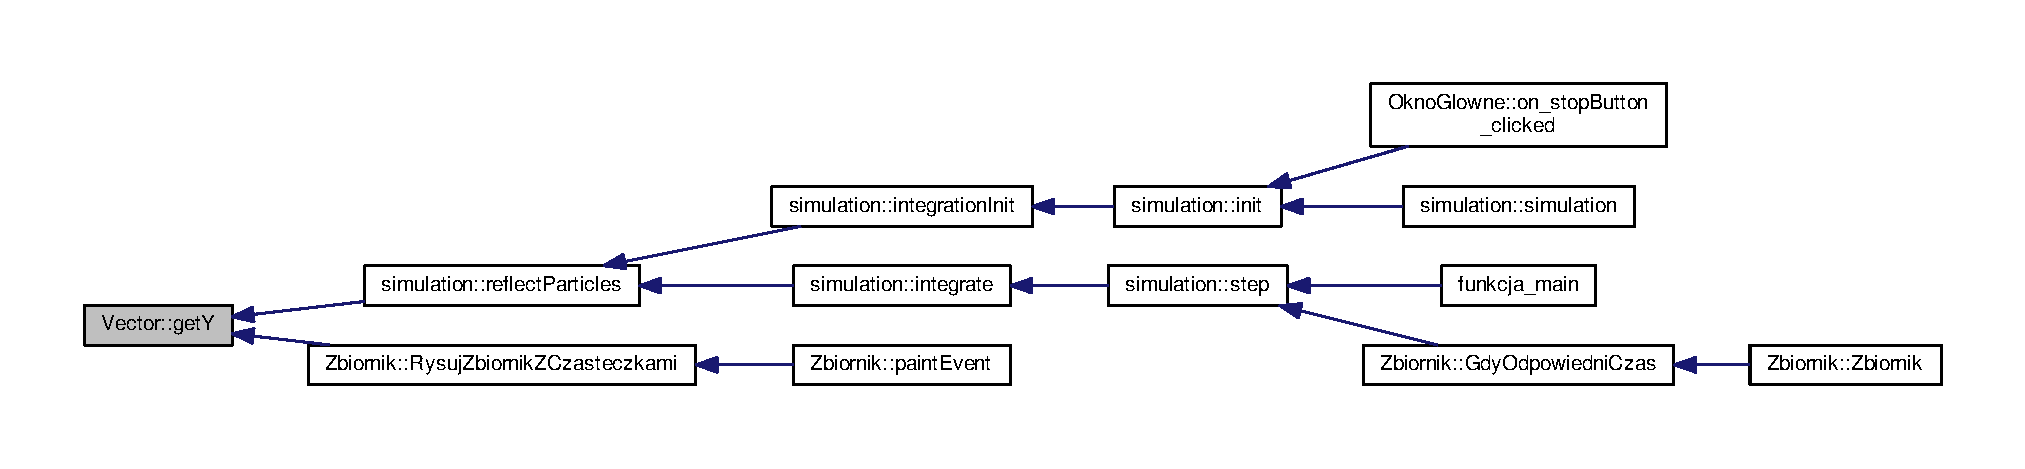
\includegraphics[width=350pt]{class_vector_a86293fe7a035979fd252be6071488b6a_icgraph}
\end{center}
\end{figure}


\hypertarget{class_vector_ab0cc77ce300a60de0ab734555886ad5d}{}\index{Vector@{Vector}!get\+Y@{get\+Y}}
\index{get\+Y@{get\+Y}!Vector@{Vector}}
\subsubsection[{get\+Y}]{\setlength{\rightskip}{0pt plus 5cm}float\& Vector\+::get\+Y (
\begin{DoxyParamCaption}
{}
\end{DoxyParamCaption}
)\hspace{0.3cm}{\ttfamily [inline]}}\label{class_vector_ab0cc77ce300a60de0ab734555886ad5d}
\begin{DoxyReturn}{Zwraca}
druga współrzędna wektora jako stała 
\end{DoxyReturn}


Definicja w linii 42 pliku vector.\+hh.

\hypertarget{class_vector_a18d3f2110be751ac3a658016bd3dca69}{}\index{Vector@{Vector}!norm\+Squared@{norm\+Squared}}
\index{norm\+Squared@{norm\+Squared}!Vector@{Vector}}
\subsubsection[{norm\+Squared}]{\setlength{\rightskip}{0pt plus 5cm}float Vector\+::norm\+Squared (
\begin{DoxyParamCaption}
{}
\end{DoxyParamCaption}
)\hspace{0.3cm}{\ttfamily [inline]}}\label{class_vector_a18d3f2110be751ac3a658016bd3dca69}
Zwraca sumę kwadratów współrzędnych wektora \begin{DoxyReturn}{Zwraca}
wartość kwadratu normy 
\end{DoxyReturn}


Definicja w linii 105 pliku vector.\+hh.



Oto graf wywoływań tej funkcji\+:\nopagebreak
\begin{figure}[H]
\begin{center}
\leavevmode
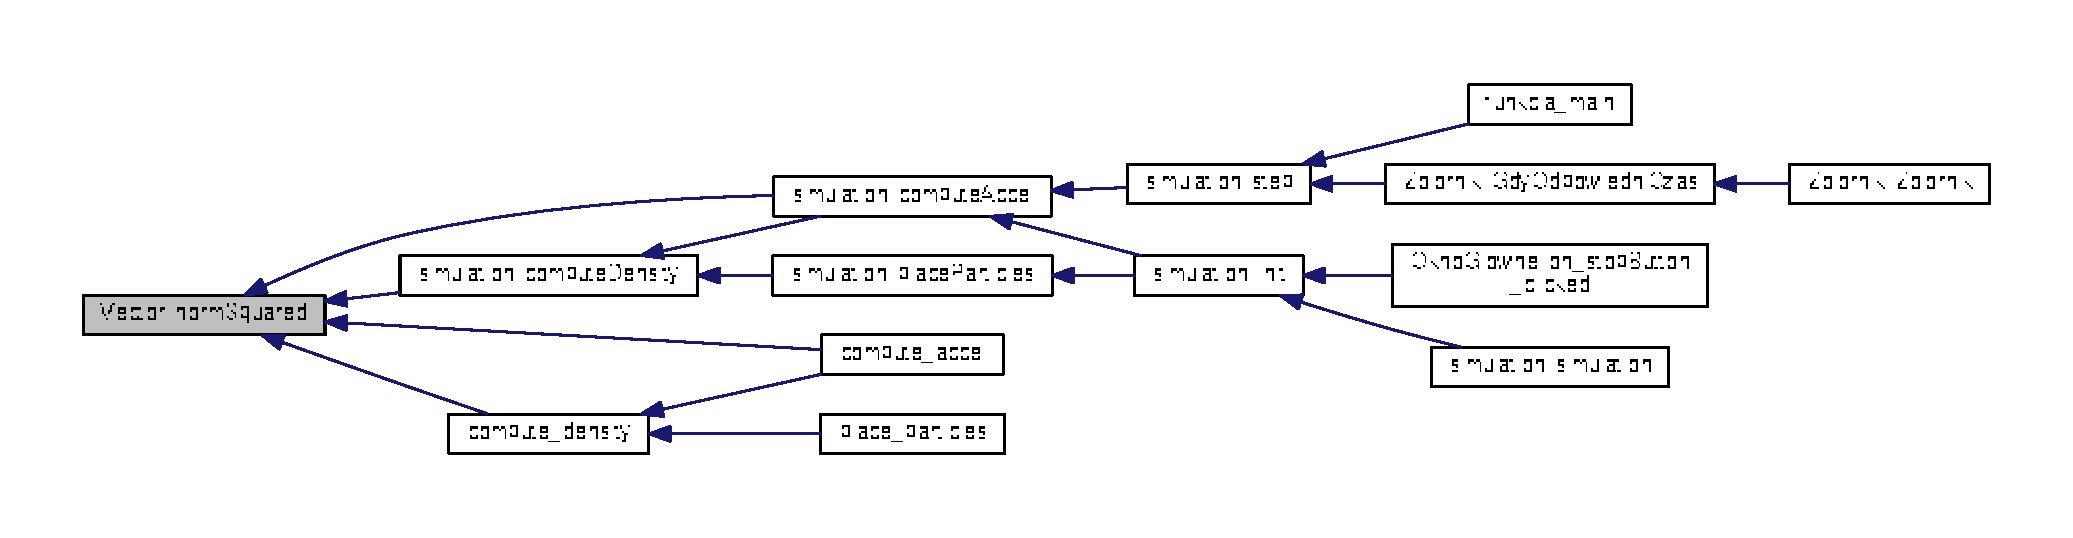
\includegraphics[width=350pt]{class_vector_a18d3f2110be751ac3a658016bd3dca69_icgraph}
\end{center}
\end{figure}


\hypertarget{class_vector_a8f0e64ee9a688803b1efce30fb0b2869}{}\index{Vector@{Vector}!operator$\ast$@{operator$\ast$}}
\index{operator$\ast$@{operator$\ast$}!Vector@{Vector}}
\subsubsection[{operator$\ast$}]{\setlength{\rightskip}{0pt plus 5cm}{\bf Vector} Vector\+::operator$\ast$ (
\begin{DoxyParamCaption}
\item[{const float \&}]{\+\_\+c}
\end{DoxyParamCaption}
) const\hspace{0.3cm}{\ttfamily [inline]}}\label{class_vector_a8f0e64ee9a688803b1efce30fb0b2869}
Skaluje wektor 
\begin{DoxyParams}[1]{Parametry}
\mbox{\tt in}  & {\em \+\_\+c} & -\/ współczynnik skalowania \\
\hline
\end{DoxyParams}
\begin{DoxyReturn}{Zwraca}
przeskalowany wektor 
\end{DoxyReturn}


Definicja w linii 90 pliku vector.\+hh.



Oto graf wywołań dla tej funkcji\+:\nopagebreak
\begin{figure}[H]
\begin{center}
\leavevmode
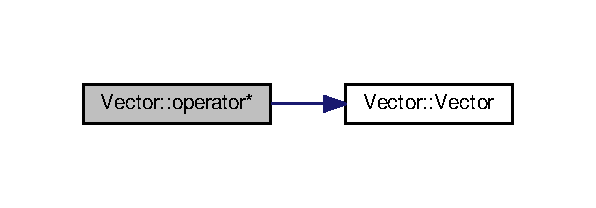
\includegraphics[width=297pt]{class_vector_a8f0e64ee9a688803b1efce30fb0b2869_cgraph}
\end{center}
\end{figure}


\hypertarget{class_vector_a91ebac6d502ca1d54645e7c711549867}{}\index{Vector@{Vector}!operator$\ast$=@{operator$\ast$=}}
\index{operator$\ast$=@{operator$\ast$=}!Vector@{Vector}}
\subsubsection[{operator$\ast$=}]{\setlength{\rightskip}{0pt plus 5cm}{\bf Vector}\& Vector\+::operator$\ast$= (
\begin{DoxyParamCaption}
\item[{const float \&}]{\+\_\+c}
\end{DoxyParamCaption}
)\hspace{0.3cm}{\ttfamily [inline]}}\label{class_vector_a91ebac6d502ca1d54645e7c711549867}
Skaluje wektor 
\begin{DoxyParams}[1]{Parametry}
\mbox{\tt in}  & {\em \+\_\+c} & -\/ współczynnik \\
\hline
\end{DoxyParams}
\begin{DoxyReturn}{Zwraca}
referencja na pierwotny obiekt 
\end{DoxyReturn}


Definicja w linii 66 pliku vector.\+hh.

\hypertarget{class_vector_aa78eb4c9e5ac236c89f0853eefa347ac}{}\index{Vector@{Vector}!operator+@{operator+}}
\index{operator+@{operator+}!Vector@{Vector}}
\subsubsection[{operator+}]{\setlength{\rightskip}{0pt plus 5cm}{\bf Vector} Vector\+::operator+ (
\begin{DoxyParamCaption}
\item[{const {\bf Vector} \&}]{\+\_\+v}
\end{DoxyParamCaption}
) const\hspace{0.3cm}{\ttfamily [inline]}}\label{class_vector_aa78eb4c9e5ac236c89f0853eefa347ac}
Dodaje wartość dwóch wektorów 
\begin{DoxyParams}[1]{Parametry}
\mbox{\tt in}  & {\em \+\_\+v} & -\/ inny wektor \\
\hline
\end{DoxyParams}
\begin{DoxyReturn}{Zwraca}
wektor będący sumą 
\end{DoxyReturn}


Definicja w linii 74 pliku vector.\+hh.



Oto graf wywołań dla tej funkcji\+:\nopagebreak
\begin{figure}[H]
\begin{center}
\leavevmode
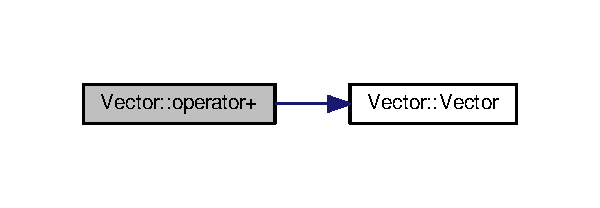
\includegraphics[width=298pt]{class_vector_aa78eb4c9e5ac236c89f0853eefa347ac_cgraph}
\end{center}
\end{figure}


\hypertarget{class_vector_a4eeab5be24ee846de3012e67a4e34820}{}\index{Vector@{Vector}!operator+=@{operator+=}}
\index{operator+=@{operator+=}!Vector@{Vector}}
\subsubsection[{operator+=}]{\setlength{\rightskip}{0pt plus 5cm}{\bf Vector}\& Vector\+::operator+= (
\begin{DoxyParamCaption}
\item[{const {\bf Vector} \&}]{\+\_\+v}
\end{DoxyParamCaption}
)\hspace{0.3cm}{\ttfamily [inline]}}\label{class_vector_a4eeab5be24ee846de3012e67a4e34820}
Dodaje wartość innego wektora do klasy 
\begin{DoxyParams}[1]{Parametry}
\mbox{\tt in}  & {\em \+\_\+v} & -\/ inny wektor \\
\hline
\end{DoxyParams}
\begin{DoxyReturn}{Zwraca}
referencja na pierwotny obiekt 
\end{DoxyReturn}


Definicja w linii 50 pliku vector.\+hh.

\hypertarget{class_vector_a94b6fde82bef6532c00358a0af448fc1}{}\index{Vector@{Vector}!operator-\/@{operator-\/}}
\index{operator-\/@{operator-\/}!Vector@{Vector}}
\subsubsection[{operator-\/}]{\setlength{\rightskip}{0pt plus 5cm}{\bf Vector} Vector\+::operator-\/ (
\begin{DoxyParamCaption}
\item[{const {\bf Vector} \&}]{\+\_\+v}
\end{DoxyParamCaption}
) const\hspace{0.3cm}{\ttfamily [inline]}}\label{class_vector_a94b6fde82bef6532c00358a0af448fc1}
Odejmuje wartość innego wektora od klasy 
\begin{DoxyParams}[1]{Parametry}
\mbox{\tt in}  & {\em \+\_\+v} & -\/ inny wektor \\
\hline
\end{DoxyParams}
\begin{DoxyReturn}{Zwraca}
wektor będący różnicą 
\end{DoxyReturn}


Definicja w linii 82 pliku vector.\+hh.



Oto graf wywołań dla tej funkcji\+:\nopagebreak
\begin{figure}[H]
\begin{center}
\leavevmode
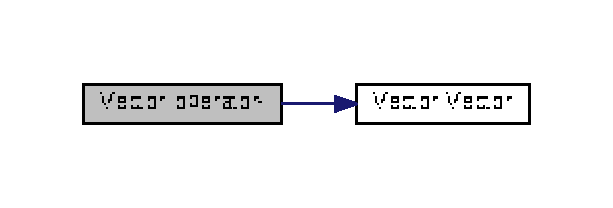
\includegraphics[width=294pt]{class_vector_a94b6fde82bef6532c00358a0af448fc1_cgraph}
\end{center}
\end{figure}


\hypertarget{class_vector_aaaf87dbf15cd9492aa0c11874ae5afef}{}\index{Vector@{Vector}!operator-\/=@{operator-\/=}}
\index{operator-\/=@{operator-\/=}!Vector@{Vector}}
\subsubsection[{operator-\/=}]{\setlength{\rightskip}{0pt plus 5cm}{\bf Vector}\& Vector\+::operator-\/= (
\begin{DoxyParamCaption}
\item[{const {\bf Vector} \&}]{\+\_\+v}
\end{DoxyParamCaption}
)\hspace{0.3cm}{\ttfamily [inline]}}\label{class_vector_aaaf87dbf15cd9492aa0c11874ae5afef}
Odejmuje wartość innego wektora od klasy 
\begin{DoxyParams}[1]{Parametry}
\mbox{\tt in}  & {\em \+\_\+v} & -\/ inny wektor \\
\hline
\end{DoxyParams}
\begin{DoxyReturn}{Zwraca}
referencja na pierwotny obiekt 
\end{DoxyReturn}


Definicja w linii 58 pliku vector.\+hh.

\hypertarget{class_vector_ad44f6d9721d9584e7f847e449df73e11}{}\index{Vector@{Vector}!operator=@{operator=}}
\index{operator=@{operator=}!Vector@{Vector}}
\subsubsection[{operator=}]{\setlength{\rightskip}{0pt plus 5cm}{\bf Vector}\& Vector\+::operator= (
\begin{DoxyParamCaption}
\item[{const {\bf Vector} \&}]{\+\_\+v}
\end{DoxyParamCaption}
)\hspace{0.3cm}{\ttfamily [inline]}}\label{class_vector_ad44f6d9721d9584e7f847e449df73e11}
Przypisuje współrzędne innego wektora do klasy 
\begin{DoxyParams}[1]{Parametry}
\mbox{\tt in}  & {\em \+\_\+v} & -\/ inny wektor \\
\hline
\end{DoxyParams}
\begin{DoxyReturn}{Zwraca}
referencja na pierwotny obiekt 
\end{DoxyReturn}


Definicja w linii 98 pliku vector.\+hh.



\subsection{Dokumentacja przyjaciół i funkcji związanych}
\hypertarget{class_vector_a7973d0032b0df4c3ab89e1da167b86a9}{}\index{Vector@{Vector}!operator$<$$<$@{operator$<$$<$}}
\index{operator$<$$<$@{operator$<$$<$}!Vector@{Vector}}
\subsubsection[{operator$<$$<$}]{\setlength{\rightskip}{0pt plus 5cm}std\+::ostream\& operator$<$$<$ (
\begin{DoxyParamCaption}
\item[{std\+::ostream \&}]{\+\_\+os, }
\item[{const {\bf Vector} \&}]{\+\_\+s}
\end{DoxyParamCaption}
)\hspace{0.3cm}{\ttfamily [friend]}}\label{class_vector_a7973d0032b0df4c3ab89e1da167b86a9}


Definicja w linii 2 pliku vector.\+cpp.



\subsection{Dokumentacja atrybutów składowych}
\hypertarget{class_vector_aca49165049a1e21ae47afcfc078819ed}{}\index{Vector@{Vector}!x@{x}}
\index{x@{x}!Vector@{Vector}}
\subsubsection[{x}]{\setlength{\rightskip}{0pt plus 5cm}float Vector\+::x\hspace{0.3cm}{\ttfamily [private]}}\label{class_vector_aca49165049a1e21ae47afcfc078819ed}


Definicja w linii 12 pliku vector.\+hh.

\hypertarget{class_vector_a81be9102fca6d9beea3efef522c4c09d}{}\index{Vector@{Vector}!y@{y}}
\index{y@{y}!Vector@{Vector}}
\subsubsection[{y}]{\setlength{\rightskip}{0pt plus 5cm}float Vector\+::y\hspace{0.3cm}{\ttfamily [private]}}\label{class_vector_a81be9102fca6d9beea3efef522c4c09d}


Definicja w linii 12 pliku vector.\+hh.



Dokumentacja dla tej klasy została wygenerowana z pliku\+:\begin{DoxyCompactItemize}
\item 
\hyperlink{vector_8hh}{vector.\+hh}\end{DoxyCompactItemize}

\hypertarget{class_zbiornik}{}\section{Dokumentacja klasy Zbiornik}
\label{class_zbiornik}\index{Zbiornik@{Zbiornik}}


Klasa modelująca zbiornik.  




{\ttfamily \#include $<$zbiornik.\+hh$>$}



Diagram dziedziczenia dla Zbiornik\nopagebreak
\begin{figure}[H]
\begin{center}
\leavevmode
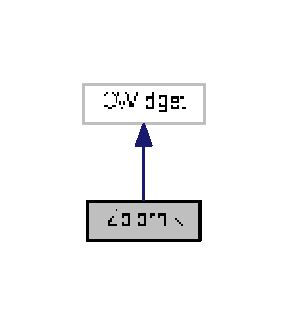
\includegraphics[width=134pt]{class_zbiornik__inherit__graph}
\end{center}
\end{figure}


Diagram współpracy dla Zbiornik\+:\nopagebreak
\begin{figure}[H]
\begin{center}
\leavevmode
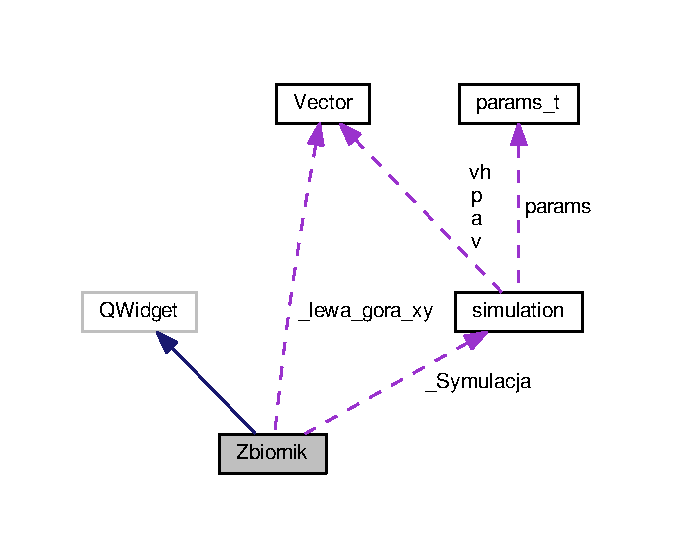
\includegraphics[width=134pt]{class_zbiornik__coll__graph}
\end{center}
\end{figure}
\subsection*{Sloty publiczne}
\begin{DoxyCompactItemize}
\item 
void \hyperlink{class_zbiornik_aa07ceb0fcbf307f0aa1eb75c32f3f47e}{Gdy\+Odpowiedni\+Czas} ()
\begin{DoxyCompactList}\small\item\em Slot odpowiadajacy za aktualizacje danych. . \end{DoxyCompactList}\end{DoxyCompactItemize}
\subsection*{Sygnały}
\begin{DoxyCompactItemize}
\item 
void \hyperlink{class_zbiornik_a2d92e4a46f9a5dda37ddd9948046580b}{Zglos\+Napis} (const Q\+String \&)
\begin{DoxyCompactList}\small\item\em Sygnal zglaszajacy napis. \end{DoxyCompactList}\item 
void \hyperlink{class_zbiornik_ad200a7e5bc038ad94131d1a354266889}{Zglos\+Liczbe\+Czasteczek} (const int)
\item 
void \hyperlink{class_zbiornik_a96b9ee7d80fc0f29787dc060027d2805}{Zglos\+Czas\+Symulacji} (const double)
\end{DoxyCompactItemize}
\subsection*{Metody publiczne}
\begin{DoxyCompactItemize}
\item 
\hyperlink{class_zbiornik_a52fb780bf924b89018348be8a65eaf68}{Zbiornik} (Q\+Widget $\ast$w\+Rodzic=N\+U\+L\+L)
\begin{DoxyCompactList}\small\item\em Konstruktor. \end{DoxyCompactList}\item 
virtual void \hyperlink{class_zbiornik_af7a9c185e95b92de342c6dc69f020765}{paint\+Event} (Q\+Paint\+Event $\ast$event)
\begin{DoxyCompactList}\small\item\em Wirtualna metoda paint\+Event wyrysowujaca obiekt na ekranie. \end{DoxyCompactList}\item 
void \hyperlink{class_zbiornik_ad15f40d418d9ebf261de0eabe8cc2906}{Rysuj\+Zbiornik} (Q\+Painter \&Rysownik, const int Podstawa, const int Wysokosc, const int Grubosc, const int x, const int y)
\begin{DoxyCompactList}\small\item\em Metoda rysujaca zbiornik. \end{DoxyCompactList}\item 
void \hyperlink{class_zbiornik_ad93223745351d4d18f64c5c43dfc5fdc}{Rysuj\+Czasteczke} (Q\+Painter \&Rysownik, const int Promien, const \hyperlink{class_kolor}{Kolor} R\+G\+B, const double x, const double y)
\begin{DoxyCompactList}\small\item\em Metoda rysujaca czasteczke. \end{DoxyCompactList}\item 
void \hyperlink{class_zbiornik_af831a2751191eab54fb6438392ac6edb}{Rysuj\+Zbiornik\+Z\+Czasteczkami} (Q\+Painter \&Rysownik)
\begin{DoxyCompactList}\small\item\em Metoda rysujaca zbiornik wraz z czasteczkami. \end{DoxyCompactList}\end{DoxyCompactItemize}
\subsection*{Atrybuty publiczne}
\begin{DoxyCompactItemize}
\item 
std\+::list$<$ \hyperlink{class_czasteczka}{Czasteczka} $>$ \hyperlink{class_zbiornik_a751209f2f02a7eaf3b7a3283d8fcd3ad}{Czasteczki}
\begin{DoxyCompactList}\small\item\em Lista wszystkich czasteczek. \end{DoxyCompactList}\end{DoxyCompactItemize}
\subsection*{Atrybuty prywatne}
\begin{DoxyCompactItemize}
\item 
Q\+Timer \hyperlink{class_zbiornik_a5ca8ac1357ef59110d4a9e12aae2bd99}{\+\_\+\+Stoper}
\begin{DoxyCompactList}\small\item\em Miernik czasu. \end{DoxyCompactList}\end{DoxyCompactItemize}


\subsection{Opis szczegółowy}
Dzieki tej klasie mozliwe jest wyrysowywanie na ekranie zbiornika. 

Definicja w linii 77 pliku zbiornik.\+hh.



\subsection{Dokumentacja konstruktora i destruktora}
\hypertarget{class_zbiornik_a52fb780bf924b89018348be8a65eaf68}{}\index{Zbiornik@{Zbiornik}!Zbiornik@{Zbiornik}}
\index{Zbiornik@{Zbiornik}!Zbiornik@{Zbiornik}}
\subsubsection[{Zbiornik}]{\setlength{\rightskip}{0pt plus 5cm}Zbiornik\+::\+Zbiornik (
\begin{DoxyParamCaption}
\item[{Q\+Widget $\ast$}]{w\+Rodzic = {\ttfamily NULL}}
\end{DoxyParamCaption}
)}\label{class_zbiornik_a52fb780bf924b89018348be8a65eaf68}
Konstruktor parametryczny. 
\begin{DoxyParams}[1]{Parametry}
\mbox{\tt in,out}  & {\em w\+Rodzic} & -\/ wskaznik na rodzica \\
\hline
\end{DoxyParams}


Definicja w linii 18 pliku zbiornik.\+cpp.



Oto graf wywołań dla tej funkcji\+:
\nopagebreak
\begin{figure}[H]
\begin{center}
\leavevmode
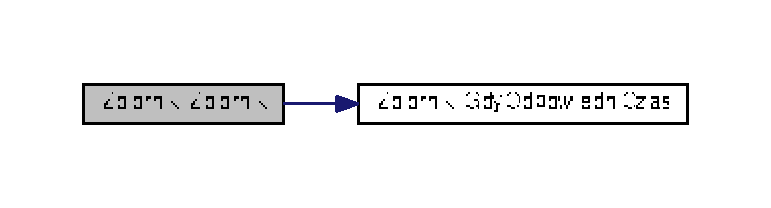
\includegraphics[width=350pt]{class_zbiornik_a52fb780bf924b89018348be8a65eaf68_cgraph}
\end{center}
\end{figure}




\subsection{Dokumentacja funkcji składowych}
\hypertarget{class_zbiornik_aa07ceb0fcbf307f0aa1eb75c32f3f47e}{}\index{Zbiornik@{Zbiornik}!Gdy\+Odpowiedni\+Czas@{Gdy\+Odpowiedni\+Czas}}
\index{Gdy\+Odpowiedni\+Czas@{Gdy\+Odpowiedni\+Czas}!Zbiornik@{Zbiornik}}
\subsubsection[{Gdy\+Odpowiedni\+Czas}]{\setlength{\rightskip}{0pt plus 5cm}void Zbiornik\+::\+Gdy\+Odpowiedni\+Czas (
\begin{DoxyParamCaption}
{}
\end{DoxyParamCaption}
)\hspace{0.3cm}{\ttfamily [slot]}}\label{class_zbiornik_aa07ceb0fcbf307f0aa1eb75c32f3f47e}
Odpowiada za uaktualnienie zbiornika w odpowiednich momentach. 

Definicja w linii 84 pliku zbiornik.\+cpp.



Oto graf wywoływań tej funkcji\+:
\nopagebreak
\begin{figure}[H]
\begin{center}
\leavevmode
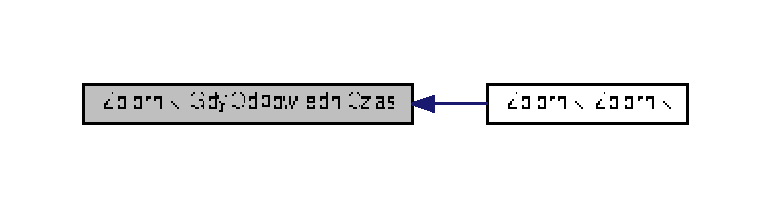
\includegraphics[width=350pt]{class_zbiornik_aa07ceb0fcbf307f0aa1eb75c32f3f47e_icgraph}
\end{center}
\end{figure}


\hypertarget{class_zbiornik_af7a9c185e95b92de342c6dc69f020765}{}\index{Zbiornik@{Zbiornik}!paint\+Event@{paint\+Event}}
\index{paint\+Event@{paint\+Event}!Zbiornik@{Zbiornik}}
\subsubsection[{paint\+Event}]{\setlength{\rightskip}{0pt plus 5cm}void Zbiornik\+::paint\+Event (
\begin{DoxyParamCaption}
\item[{Q\+Paint\+Event $\ast$}]{event}
\end{DoxyParamCaption}
)\hspace{0.3cm}{\ttfamily [virtual]}}\label{class_zbiornik_af7a9c185e95b92de342c6dc69f020765}
Odziedziczona wirtualna metoda paint\+Event. 
\begin{DoxyParams}[1]{Parametry}
\mbox{\tt in,out}  & {\em event} & -\/ wskaznik obiekt klasy Q\+Paint\+Event \\
\hline
\end{DoxyParams}


Definicja w linii 69 pliku zbiornik.\+cpp.



Oto graf wywołań dla tej funkcji\+:
\nopagebreak
\begin{figure}[H]
\begin{center}
\leavevmode
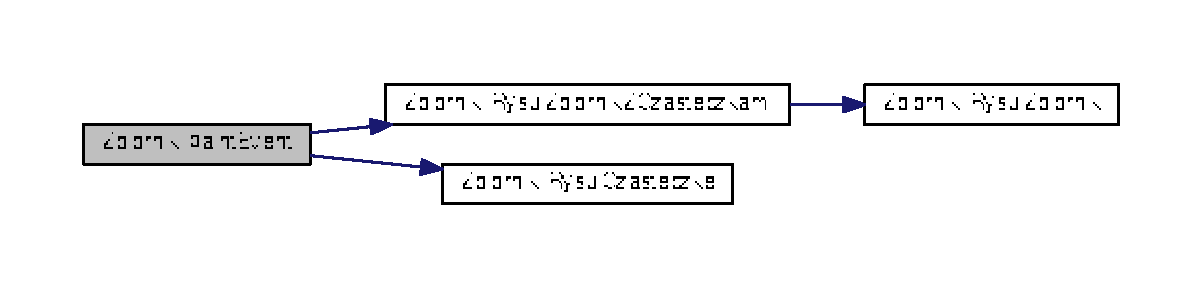
\includegraphics[width=350pt]{class_zbiornik_af7a9c185e95b92de342c6dc69f020765_cgraph}
\end{center}
\end{figure}


\hypertarget{class_zbiornik_ad93223745351d4d18f64c5c43dfc5fdc}{}\index{Zbiornik@{Zbiornik}!Rysuj\+Czasteczke@{Rysuj\+Czasteczke}}
\index{Rysuj\+Czasteczke@{Rysuj\+Czasteczke}!Zbiornik@{Zbiornik}}
\subsubsection[{Rysuj\+Czasteczke}]{\setlength{\rightskip}{0pt plus 5cm}void Zbiornik\+::\+Rysuj\+Czasteczke (
\begin{DoxyParamCaption}
\item[{Q\+Painter \&}]{Rysownik, }
\item[{const int}]{Promien, }
\item[{const {\bf Kolor}}]{R\+G\+B, }
\item[{const double}]{x, }
\item[{const double}]{y}
\end{DoxyParamCaption}
)}\label{class_zbiornik_ad93223745351d4d18f64c5c43dfc5fdc}
Rysuje czasteczke o zadanych parametrach 
\begin{DoxyParams}[1]{Parametry}
\mbox{\tt in,out}  & {\em Rysownik} & -\/ referencja na obiekt klasy Q\+Painter \\
\hline
\mbox{\tt in}  & {\em Promien} & -\/ promien czasteczki \\
\hline
\mbox{\tt in}  & {\em R\+G\+B} & -\/ kolor czasteczki w formacie R\+G\+B \\
\hline
\mbox{\tt in}  & {\em x} & -\/ polozenie czasteczki na osi x \\
\hline
\mbox{\tt in}  & {\em y} & -\/ polozenie czasteczki na osi y \\
\hline
\end{DoxyParams}


Definicja w linii 46 pliku zbiornik.\+cpp.



Oto graf wywoływań tej funkcji\+:
\nopagebreak
\begin{figure}[H]
\begin{center}
\leavevmode
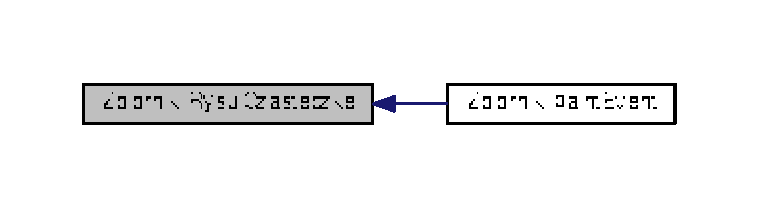
\includegraphics[width=350pt]{class_zbiornik_ad93223745351d4d18f64c5c43dfc5fdc_icgraph}
\end{center}
\end{figure}


\hypertarget{class_zbiornik_ad15f40d418d9ebf261de0eabe8cc2906}{}\index{Zbiornik@{Zbiornik}!Rysuj\+Zbiornik@{Rysuj\+Zbiornik}}
\index{Rysuj\+Zbiornik@{Rysuj\+Zbiornik}!Zbiornik@{Zbiornik}}
\subsubsection[{Rysuj\+Zbiornik}]{\setlength{\rightskip}{0pt plus 5cm}void Zbiornik\+::\+Rysuj\+Zbiornik (
\begin{DoxyParamCaption}
\item[{Q\+Painter \&}]{Rysownik, }
\item[{const int}]{Podstawa, }
\item[{const int}]{Wysokosc, }
\item[{const int}]{Grubosc, }
\item[{const int}]{x, }
\item[{const int}]{y}
\end{DoxyParamCaption}
)}\label{class_zbiornik_ad15f40d418d9ebf261de0eabe8cc2906}
Rysuje zbiornik o zadanych parametrach. 
\begin{DoxyParams}[1]{Parametry}
\mbox{\tt in,out}  & {\em Rysownik} & -\/ referencja na obiekt klasy Q\+Painter \\
\hline
\mbox{\tt in}  & {\em Podstawa} & -\/ dlugosc podstawy zbiornika \\
\hline
\mbox{\tt in}  & {\em Wysokosc} & -\/ wysokosc zbiornika \\
\hline
\mbox{\tt in}  & {\em Grubosc} & -\/ grubosc wyrysowywanego odcinka \\
\hline
\mbox{\tt in}  & {\em x} & -\/ polozenie lewego gornego punktu zbiornika na osi x \\
\hline
\mbox{\tt in}  & {\em y} & -\/ polozenie lewego gornego punktu zbiornika na osi y \\
\hline
\end{DoxyParams}


Definicja w linii 29 pliku zbiornik.\+cpp.



Oto graf wywoływań tej funkcji\+:\nopagebreak
\begin{figure}[H]
\begin{center}
\leavevmode
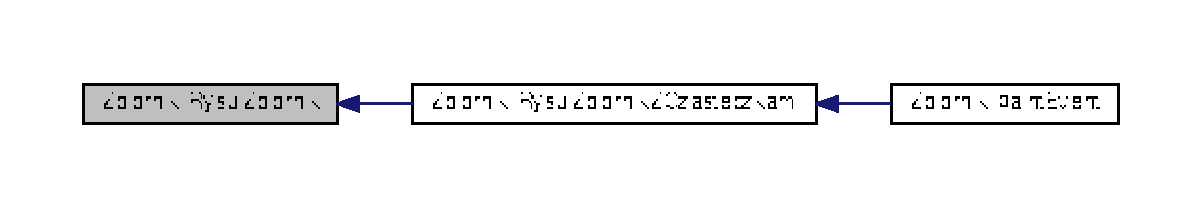
\includegraphics[width=350pt]{class_zbiornik_ad15f40d418d9ebf261de0eabe8cc2906_icgraph}
\end{center}
\end{figure}


\hypertarget{class_zbiornik_af831a2751191eab54fb6438392ac6edb}{}\index{Zbiornik@{Zbiornik}!Rysuj\+Zbiornik\+Z\+Czasteczkami@{Rysuj\+Zbiornik\+Z\+Czasteczkami}}
\index{Rysuj\+Zbiornik\+Z\+Czasteczkami@{Rysuj\+Zbiornik\+Z\+Czasteczkami}!Zbiornik@{Zbiornik}}
\subsubsection[{Rysuj\+Zbiornik\+Z\+Czasteczkami}]{\setlength{\rightskip}{0pt plus 5cm}void Zbiornik\+::\+Rysuj\+Zbiornik\+Z\+Czasteczkami (
\begin{DoxyParamCaption}
\item[{Q\+Painter \&}]{Rysownik}
\end{DoxyParamCaption}
)}\label{class_zbiornik_af831a2751191eab54fb6438392ac6edb}
Rysuje zbiornik oraz czasteczki. 
\begin{DoxyParams}[1]{Parametry}
\mbox{\tt in,out}  & {\em Rysownik} & -\/ referencja na obiekt klasy Q\+Painter \\
\hline
\end{DoxyParams}


Definicja w linii 60 pliku zbiornik.\+cpp.



Oto graf wywołań dla tej funkcji\+:
\nopagebreak
\begin{figure}[H]
\begin{center}
\leavevmode
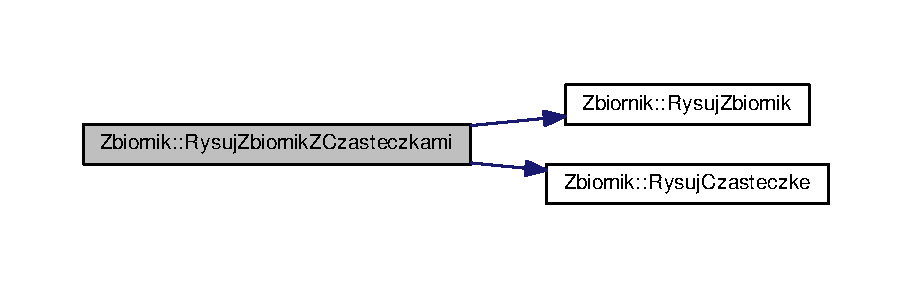
\includegraphics[width=350pt]{class_zbiornik_af831a2751191eab54fb6438392ac6edb_cgraph}
\end{center}
\end{figure}




Oto graf wywoływań tej funkcji\+:\nopagebreak
\begin{figure}[H]
\begin{center}
\leavevmode
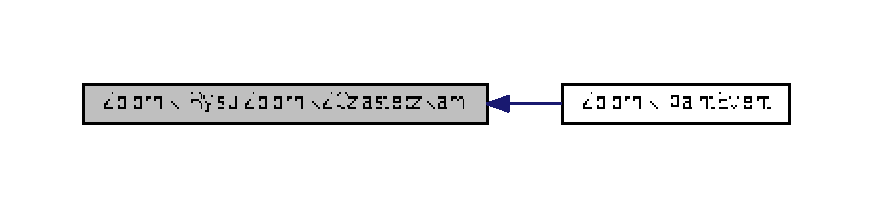
\includegraphics[width=350pt]{class_zbiornik_af831a2751191eab54fb6438392ac6edb_icgraph}
\end{center}
\end{figure}


\hypertarget{class_zbiornik_a96b9ee7d80fc0f29787dc060027d2805}{}\index{Zbiornik@{Zbiornik}!Zglos\+Czas\+Symulacji@{Zglos\+Czas\+Symulacji}}
\index{Zglos\+Czas\+Symulacji@{Zglos\+Czas\+Symulacji}!Zbiornik@{Zbiornik}}
\subsubsection[{Zglos\+Czas\+Symulacji}]{\setlength{\rightskip}{0pt plus 5cm}void Zbiornik\+::\+Zglos\+Czas\+Symulacji (
\begin{DoxyParamCaption}
\item[{const double}]{\+\_\+t1}
\end{DoxyParamCaption}
)\hspace{0.3cm}{\ttfamily [signal]}}\label{class_zbiornik_a96b9ee7d80fc0f29787dc060027d2805}


Definicja w linii 119 pliku moc\+\_\+zbiornik.\+cpp.

\hypertarget{class_zbiornik_ad200a7e5bc038ad94131d1a354266889}{}\index{Zbiornik@{Zbiornik}!Zglos\+Liczbe\+Czasteczek@{Zglos\+Liczbe\+Czasteczek}}
\index{Zglos\+Liczbe\+Czasteczek@{Zglos\+Liczbe\+Czasteczek}!Zbiornik@{Zbiornik}}
\subsubsection[{Zglos\+Liczbe\+Czasteczek}]{\setlength{\rightskip}{0pt plus 5cm}void Zbiornik\+::\+Zglos\+Liczbe\+Czasteczek (
\begin{DoxyParamCaption}
\item[{const int}]{\+\_\+t1}
\end{DoxyParamCaption}
)\hspace{0.3cm}{\ttfamily [signal]}}\label{class_zbiornik_ad200a7e5bc038ad94131d1a354266889}


Definicja w linii 112 pliku moc\+\_\+zbiornik.\+cpp.

\hypertarget{class_zbiornik_a2d92e4a46f9a5dda37ddd9948046580b}{}\index{Zbiornik@{Zbiornik}!Zglos\+Napis@{Zglos\+Napis}}
\index{Zglos\+Napis@{Zglos\+Napis}!Zbiornik@{Zbiornik}}
\subsubsection[{Zglos\+Napis}]{\setlength{\rightskip}{0pt plus 5cm}void Zbiornik\+::\+Zglos\+Napis (
\begin{DoxyParamCaption}
\item[{const Q\+String \&}]{\+\_\+t1}
\end{DoxyParamCaption}
)\hspace{0.3cm}{\ttfamily [signal]}}\label{class_zbiornik_a2d92e4a46f9a5dda37ddd9948046580b}
Sygnal zglaszajacy napis do odpowiedniego slotu. 
\begin{DoxyParams}[1]{Parametry}
\mbox{\tt in}  & {\em \+\_\+t1} & -\/ napis do zgloszenia \\
\hline
\end{DoxyParams}


Definicja w linii 105 pliku moc\+\_\+zbiornik.\+cpp.



\subsection{Dokumentacja atrybutów składowych}
\hypertarget{class_zbiornik_a5ca8ac1357ef59110d4a9e12aae2bd99}{}\index{Zbiornik@{Zbiornik}!\+\_\+\+Stoper@{\+\_\+\+Stoper}}
\index{\+\_\+\+Stoper@{\+\_\+\+Stoper}!Zbiornik@{Zbiornik}}
\subsubsection[{\+\_\+\+Stoper}]{\setlength{\rightskip}{0pt plus 5cm}Q\+Timer Zbiornik\+::\+\_\+\+Stoper\hspace{0.3cm}{\ttfamily [private]}}\label{class_zbiornik_a5ca8ac1357ef59110d4a9e12aae2bd99}
Miernik czasu. 

Definicja w linii 174 pliku zbiornik.\+hh.

\hypertarget{class_zbiornik_a751209f2f02a7eaf3b7a3283d8fcd3ad}{}\index{Zbiornik@{Zbiornik}!Czasteczki@{Czasteczki}}
\index{Czasteczki@{Czasteczki}!Zbiornik@{Zbiornik}}
\subsubsection[{Czasteczki}]{\setlength{\rightskip}{0pt plus 5cm}std\+::list$<${\bf Czasteczka}$>$ Zbiornik\+::\+Czasteczki}\label{class_zbiornik_a751209f2f02a7eaf3b7a3283d8fcd3ad}
Lista wszystkich czasteczek. 

Definicja w linii 166 pliku zbiornik.\+hh.



Dokumentacja dla tej klasy została wygenerowana z plików\+:\begin{DoxyCompactItemize}
\item 
\hyperlink{zbiornik_8hh}{zbiornik.\+hh}\item 
\hyperlink{moc__zbiornik_8cpp}{moc\+\_\+zbiornik.\+cpp}\item 
\hyperlink{zbiornik_8cpp}{zbiornik.\+cpp}\end{DoxyCompactItemize}

\chapter{Dokumentacja plików}
\hypertarget{ciecz_8cpp}{\section{Dokumentacja pliku ciecz.\-cpp}
\label{ciecz_8cpp}\index{ciecz.\-cpp@{ciecz.\-cpp}}
}
{\ttfamily \#include $<$Q\-Application$>$}\\*
{\ttfamily \#include $<$Q\-Color$>$}\\*
{\ttfamily \#include $<$Q\-Painter$>$}\\*
{\ttfamily \#include $<$Q\-Status\-Bar$>$}\\*
{\ttfamily \#include $<$Q\-Time$>$}\\*
{\ttfamily \#include $<$Q\-Date$>$}\\*
{\ttfamily \#include $<$Q\-Locale$>$}\\*
{\ttfamily \#include $<$Q\-Widget$>$}\\*
{\ttfamily \#include $<$Q\-Slider$>$}\\*
{\ttfamily \#include $<$iostream$>$}\\*
{\ttfamily \#include $<$sstream$>$}\\*
{\ttfamily \#include $<$Q\-Main\-Window$>$}\\*
{\ttfamily \#include $<$Q\-Spin\-Box$>$}\\*
{\ttfamily \#include $<$Q\-Progress\-Bar$>$}\\*
{\ttfamily \#include $<$Q\-L\-C\-D\-Number$>$}\\*
{\ttfamily \#include \char`\"{}ciecz.\-hh\char`\"{}}\\*
Wykres zależności załączania dla ciecz.\-cpp\-:
\nopagebreak
\begin{figure}[H]
\begin{center}
\leavevmode
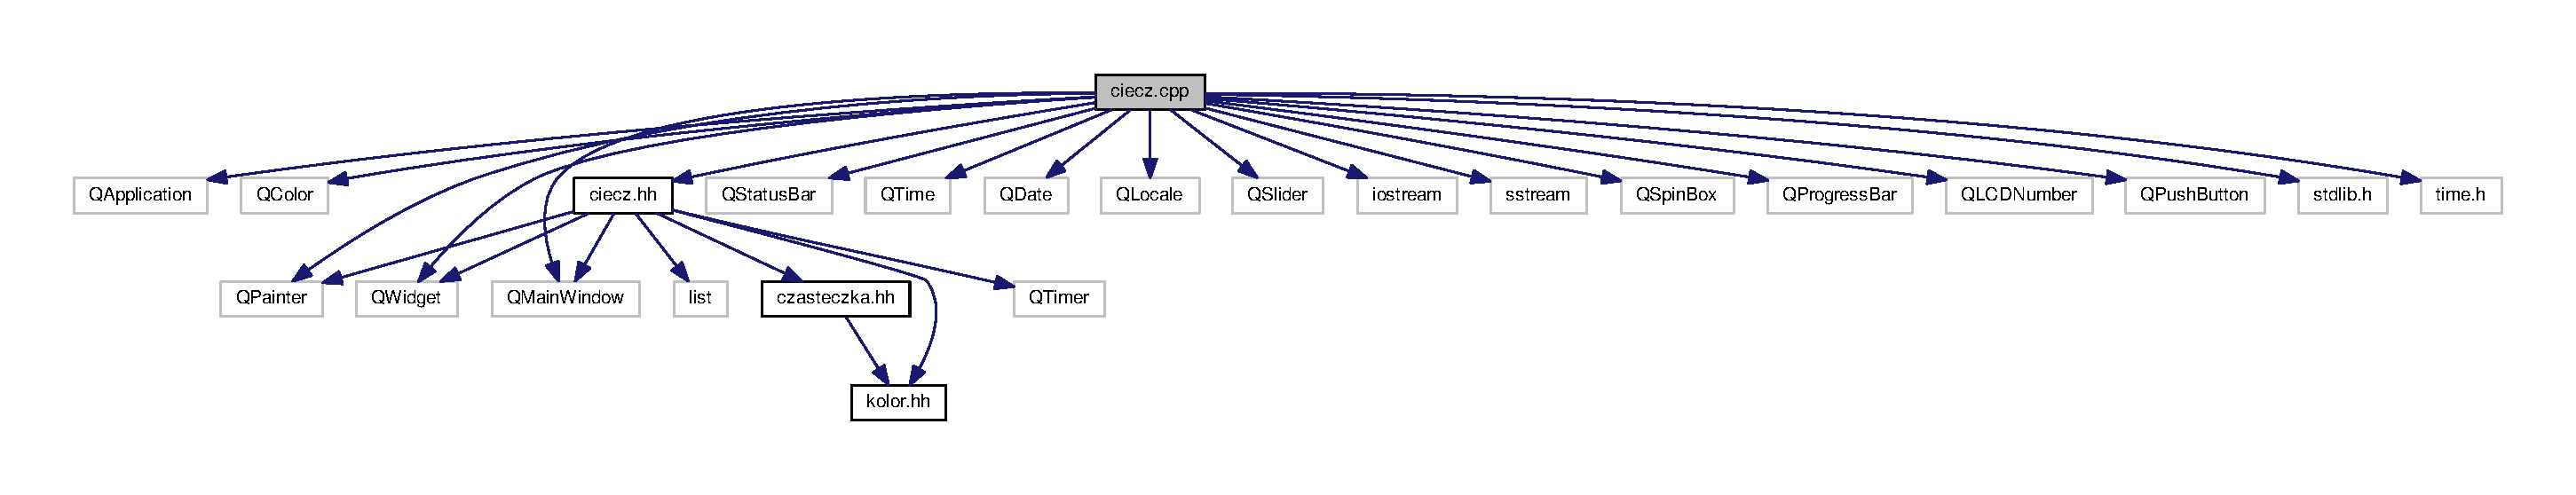
\includegraphics[width=350pt]{ciecz_8cpp__incl}
\end{center}
\end{figure}
\subsection*{Definicje}
\begin{DoxyCompactItemize}
\item 
\#define \hyperlink{ciecz_8cpp_a724df1fefe77c95e343dbf7bd36c779d}{P\-O\-D\-S\-T\-A\-W\-A}~40
\item 
\#define \hyperlink{ciecz_8cpp_a771583e9e87d083150a9a329f44c5f7e}{W\-Y\-S\-O\-K\-O\-S\-C}~50
\item 
\#define \hyperlink{ciecz_8cpp_af32bc1aae78786d4de58fb5fef677232}{G\-R\-U\-B\-O\-S\-C}~3
\end{DoxyCompactItemize}
\subsection*{Funkcje}
\begin{DoxyCompactItemize}
\item 
int \hyperlink{ciecz_8cpp_a0ddf1224851353fc92bfbff6f499fa97}{main} (int argc, char $\ast$argv\mbox{[}$\,$\mbox{]})
\end{DoxyCompactItemize}


\subsection{Dokumentacja definicji}
\hypertarget{ciecz_8cpp_af32bc1aae78786d4de58fb5fef677232}{\index{ciecz.\-cpp@{ciecz.\-cpp}!G\-R\-U\-B\-O\-S\-C@{G\-R\-U\-B\-O\-S\-C}}
\index{G\-R\-U\-B\-O\-S\-C@{G\-R\-U\-B\-O\-S\-C}!ciecz.cpp@{ciecz.\-cpp}}
\subsubsection[{G\-R\-U\-B\-O\-S\-C}]{\setlength{\rightskip}{0pt plus 5cm}\#define G\-R\-U\-B\-O\-S\-C~3}}\label{ciecz_8cpp_af32bc1aae78786d4de58fb5fef677232}


Definicja w linii 28 pliku ciecz.\-cpp.

\hypertarget{ciecz_8cpp_a724df1fefe77c95e343dbf7bd36c779d}{\index{ciecz.\-cpp@{ciecz.\-cpp}!P\-O\-D\-S\-T\-A\-W\-A@{P\-O\-D\-S\-T\-A\-W\-A}}
\index{P\-O\-D\-S\-T\-A\-W\-A@{P\-O\-D\-S\-T\-A\-W\-A}!ciecz.cpp@{ciecz.\-cpp}}
\subsubsection[{P\-O\-D\-S\-T\-A\-W\-A}]{\setlength{\rightskip}{0pt plus 5cm}\#define P\-O\-D\-S\-T\-A\-W\-A~40}}\label{ciecz_8cpp_a724df1fefe77c95e343dbf7bd36c779d}


Definicja w linii 26 pliku ciecz.\-cpp.

\hypertarget{ciecz_8cpp_a771583e9e87d083150a9a329f44c5f7e}{\index{ciecz.\-cpp@{ciecz.\-cpp}!W\-Y\-S\-O\-K\-O\-S\-C@{W\-Y\-S\-O\-K\-O\-S\-C}}
\index{W\-Y\-S\-O\-K\-O\-S\-C@{W\-Y\-S\-O\-K\-O\-S\-C}!ciecz.cpp@{ciecz.\-cpp}}
\subsubsection[{W\-Y\-S\-O\-K\-O\-S\-C}]{\setlength{\rightskip}{0pt plus 5cm}\#define W\-Y\-S\-O\-K\-O\-S\-C~50}}\label{ciecz_8cpp_a771583e9e87d083150a9a329f44c5f7e}


Definicja w linii 27 pliku ciecz.\-cpp.



\subsection{Dokumentacja funkcji}
\hypertarget{ciecz_8cpp_a0ddf1224851353fc92bfbff6f499fa97}{\index{ciecz.\-cpp@{ciecz.\-cpp}!main@{main}}
\index{main@{main}!ciecz.cpp@{ciecz.\-cpp}}
\subsubsection[{main}]{\setlength{\rightskip}{0pt plus 5cm}int main (
\begin{DoxyParamCaption}
\item[{int}]{argc, }
\item[{char $\ast$}]{argv\mbox{[}$\,$\mbox{]}}
\end{DoxyParamCaption}
)}}\label{ciecz_8cpp_a0ddf1224851353fc92bfbff6f499fa97}


Definicja w linii 87 pliku ciecz.\-cpp.


\hypertarget{ciecz_8hh}{\section{Dokumentacja pliku ciecz.\-hh}
\label{ciecz_8hh}\index{ciecz.\-hh@{ciecz.\-hh}}
}


\hyperlink{class_kanwa}{Kanwa} dla pozostalych widgetow. Jest miejscem dla umieszczania innych widgetow.  


{\ttfamily \#include $<$Q\-Widget$>$}\\*
{\ttfamily \#include $<$Q\-Main\-Window$>$}\\*
{\ttfamily \#include $<$Q\-Timer$>$}\\*
{\ttfamily \#include $<$Q\-Painter$>$}\\*
Wykres zależności załączania dla ciecz.\-hh\-:
\nopagebreak
\begin{figure}[H]
\begin{center}
\leavevmode
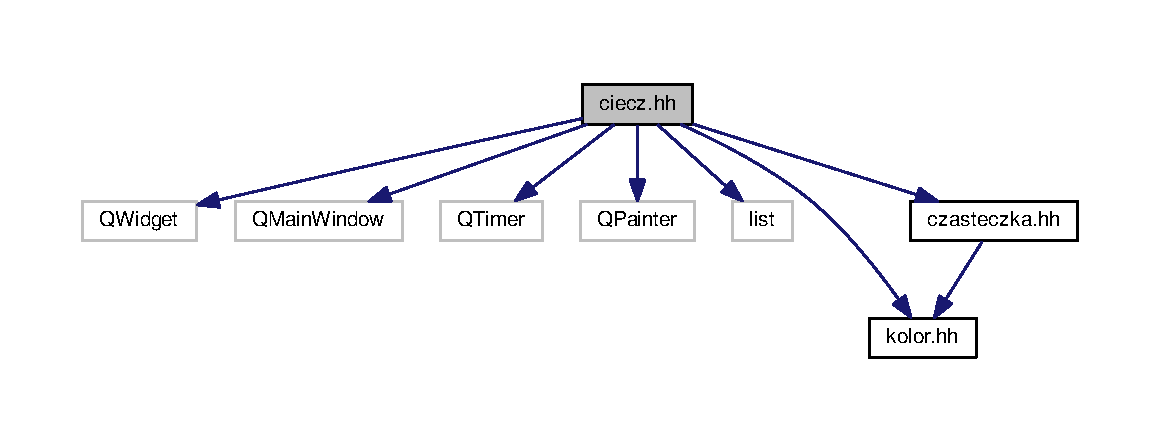
\includegraphics[width=350pt]{ciecz_8hh__incl}
\end{center}
\end{figure}
Ten wykres pokazuje, które pliki bezpośrednio lub pośrednio załączają ten plik\-:
\nopagebreak
\begin{figure}[H]
\begin{center}
\leavevmode
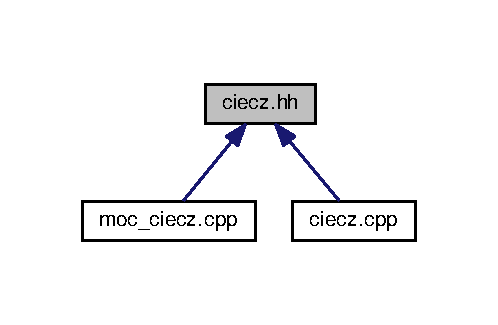
\includegraphics[width=239pt]{ciecz_8hh__dep__incl}
\end{center}
\end{figure}
\subsection*{Komponenty}
\begin{DoxyCompactItemize}
\item 
class \hyperlink{class_kanwa}{Kanwa}
\item 
class \hyperlink{class_okno_glowne}{Okno\-Glowne}
\item 
class \hyperlink{class_zbiornik}{Zbiornik}
\end{DoxyCompactItemize}


\subsection{Opis szczegółowy}
Klasa rysujaca zbiornik. Dzieki tej klasie wyrysowywany jest zbiornik na ekranie.

Główne okno aplikacji. Wyswietlane jest jako okno glowne aplikacji.

Definicja w pliku \hyperlink{ciecz_8hh_source}{ciecz.\-hh}.


\hypertarget{moc__ciecz_8cpp}{\section{Dokumentacja pliku moc\-\_\-ciecz.\-cpp}
\label{moc__ciecz_8cpp}\index{moc\-\_\-ciecz.\-cpp@{moc\-\_\-ciecz.\-cpp}}
}
{\ttfamily \#include \char`\"{}../inc/ciecz.\-hh\char`\"{}}\\*
Wykres zależności załączania dla moc\-\_\-ciecz.\-cpp\-:
\nopagebreak
\begin{figure}[H]
\begin{center}
\leavevmode
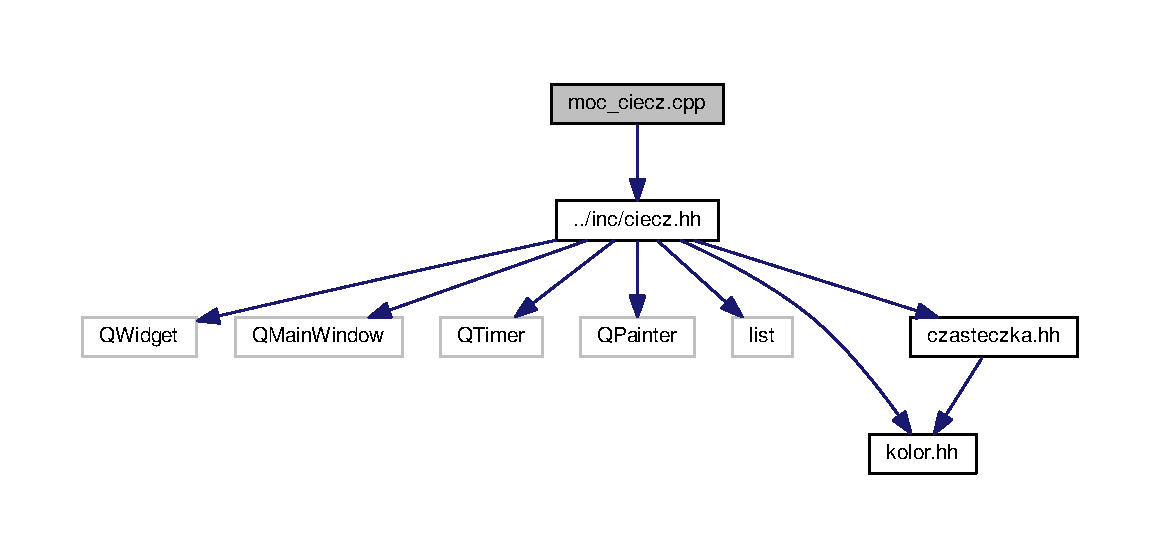
\includegraphics[width=350pt]{moc__ciecz_8cpp__incl}
\end{center}
\end{figure}

\hypertarget{strona_8dox}{}\section{Dokumentacja pliku strona.\+dox}
\label{strona_8dox}\index{strona.\+dox@{strona.\+dox}}

\hypertarget{vector_8hh}{}\section{Dokumentacja pliku vector.\+hh}
\label{vector_8hh}\index{vector.\+hh@{vector.\+hh}}
{\ttfamily \#include $<$iostream$>$}\\*
Wykres zależności załączania dla vector.\+hh\+:\nopagebreak
\begin{figure}[H]
\begin{center}
\leavevmode
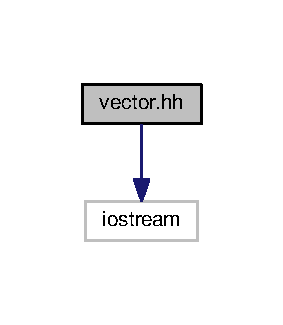
\includegraphics[width=140pt]{vector_8hh__incl}
\end{center}
\end{figure}
Ten wykres pokazuje, które pliki bezpośrednio lub pośrednio załączają ten plik\+:\nopagebreak
\begin{figure}[H]
\begin{center}
\leavevmode
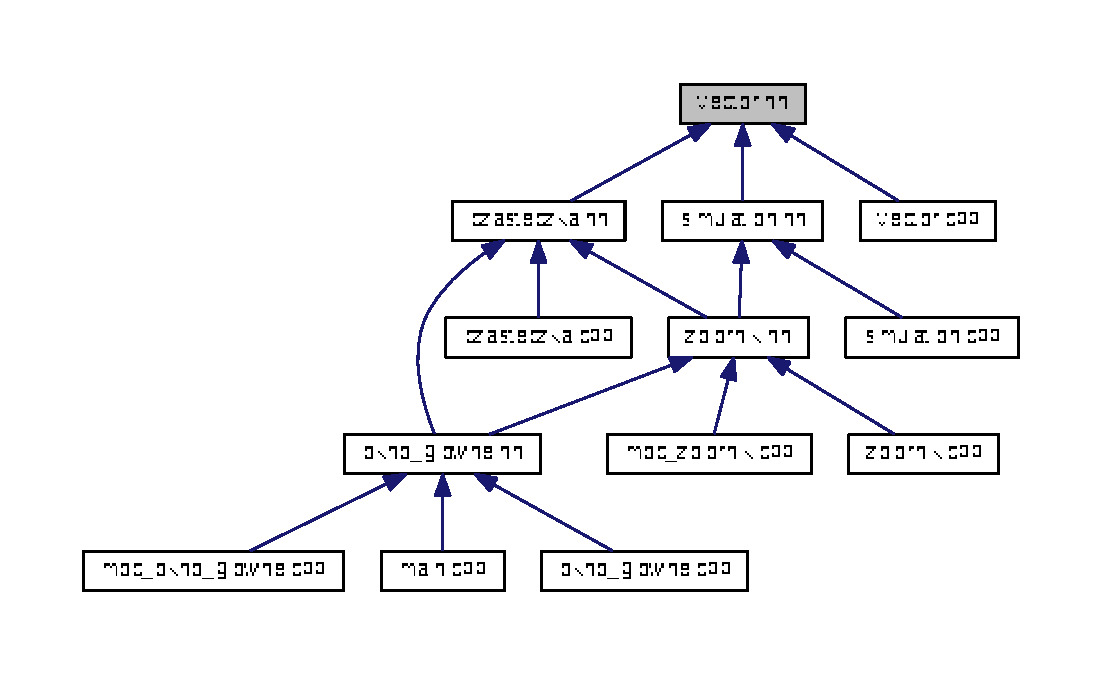
\includegraphics[width=350pt]{vector_8hh__dep__incl}
\end{center}
\end{figure}
\subsection*{Komponenty}
\begin{DoxyCompactItemize}
\item 
class \hyperlink{class_vector}{Vector}
\begin{DoxyCompactList}\small\item\em klasa \hyperlink{class_vector}{Vector} \end{DoxyCompactList}\end{DoxyCompactItemize}

%--- End generated contents ---

% Index
\newpage
\phantomsection
\addcontentsline{toc}{chapter}{Indeks}
\printindex

\end{document}
